% anhang.tex
\chapter{Appendix}
\label{ch:apdx}
\section{Additional Experiment Plots}
Here we show the remaining plots from the experiments presented in \autoref{chapter:ch5}.
The experiments are ordered by data set, regularization and bound. 
\label{sec:apdx:exp}

    \begin{landscape}
    \begin{figure}
        \centering
        \textbf{Susy, No regularization, Bound $\epsilon=0.05$}\par\medskip
        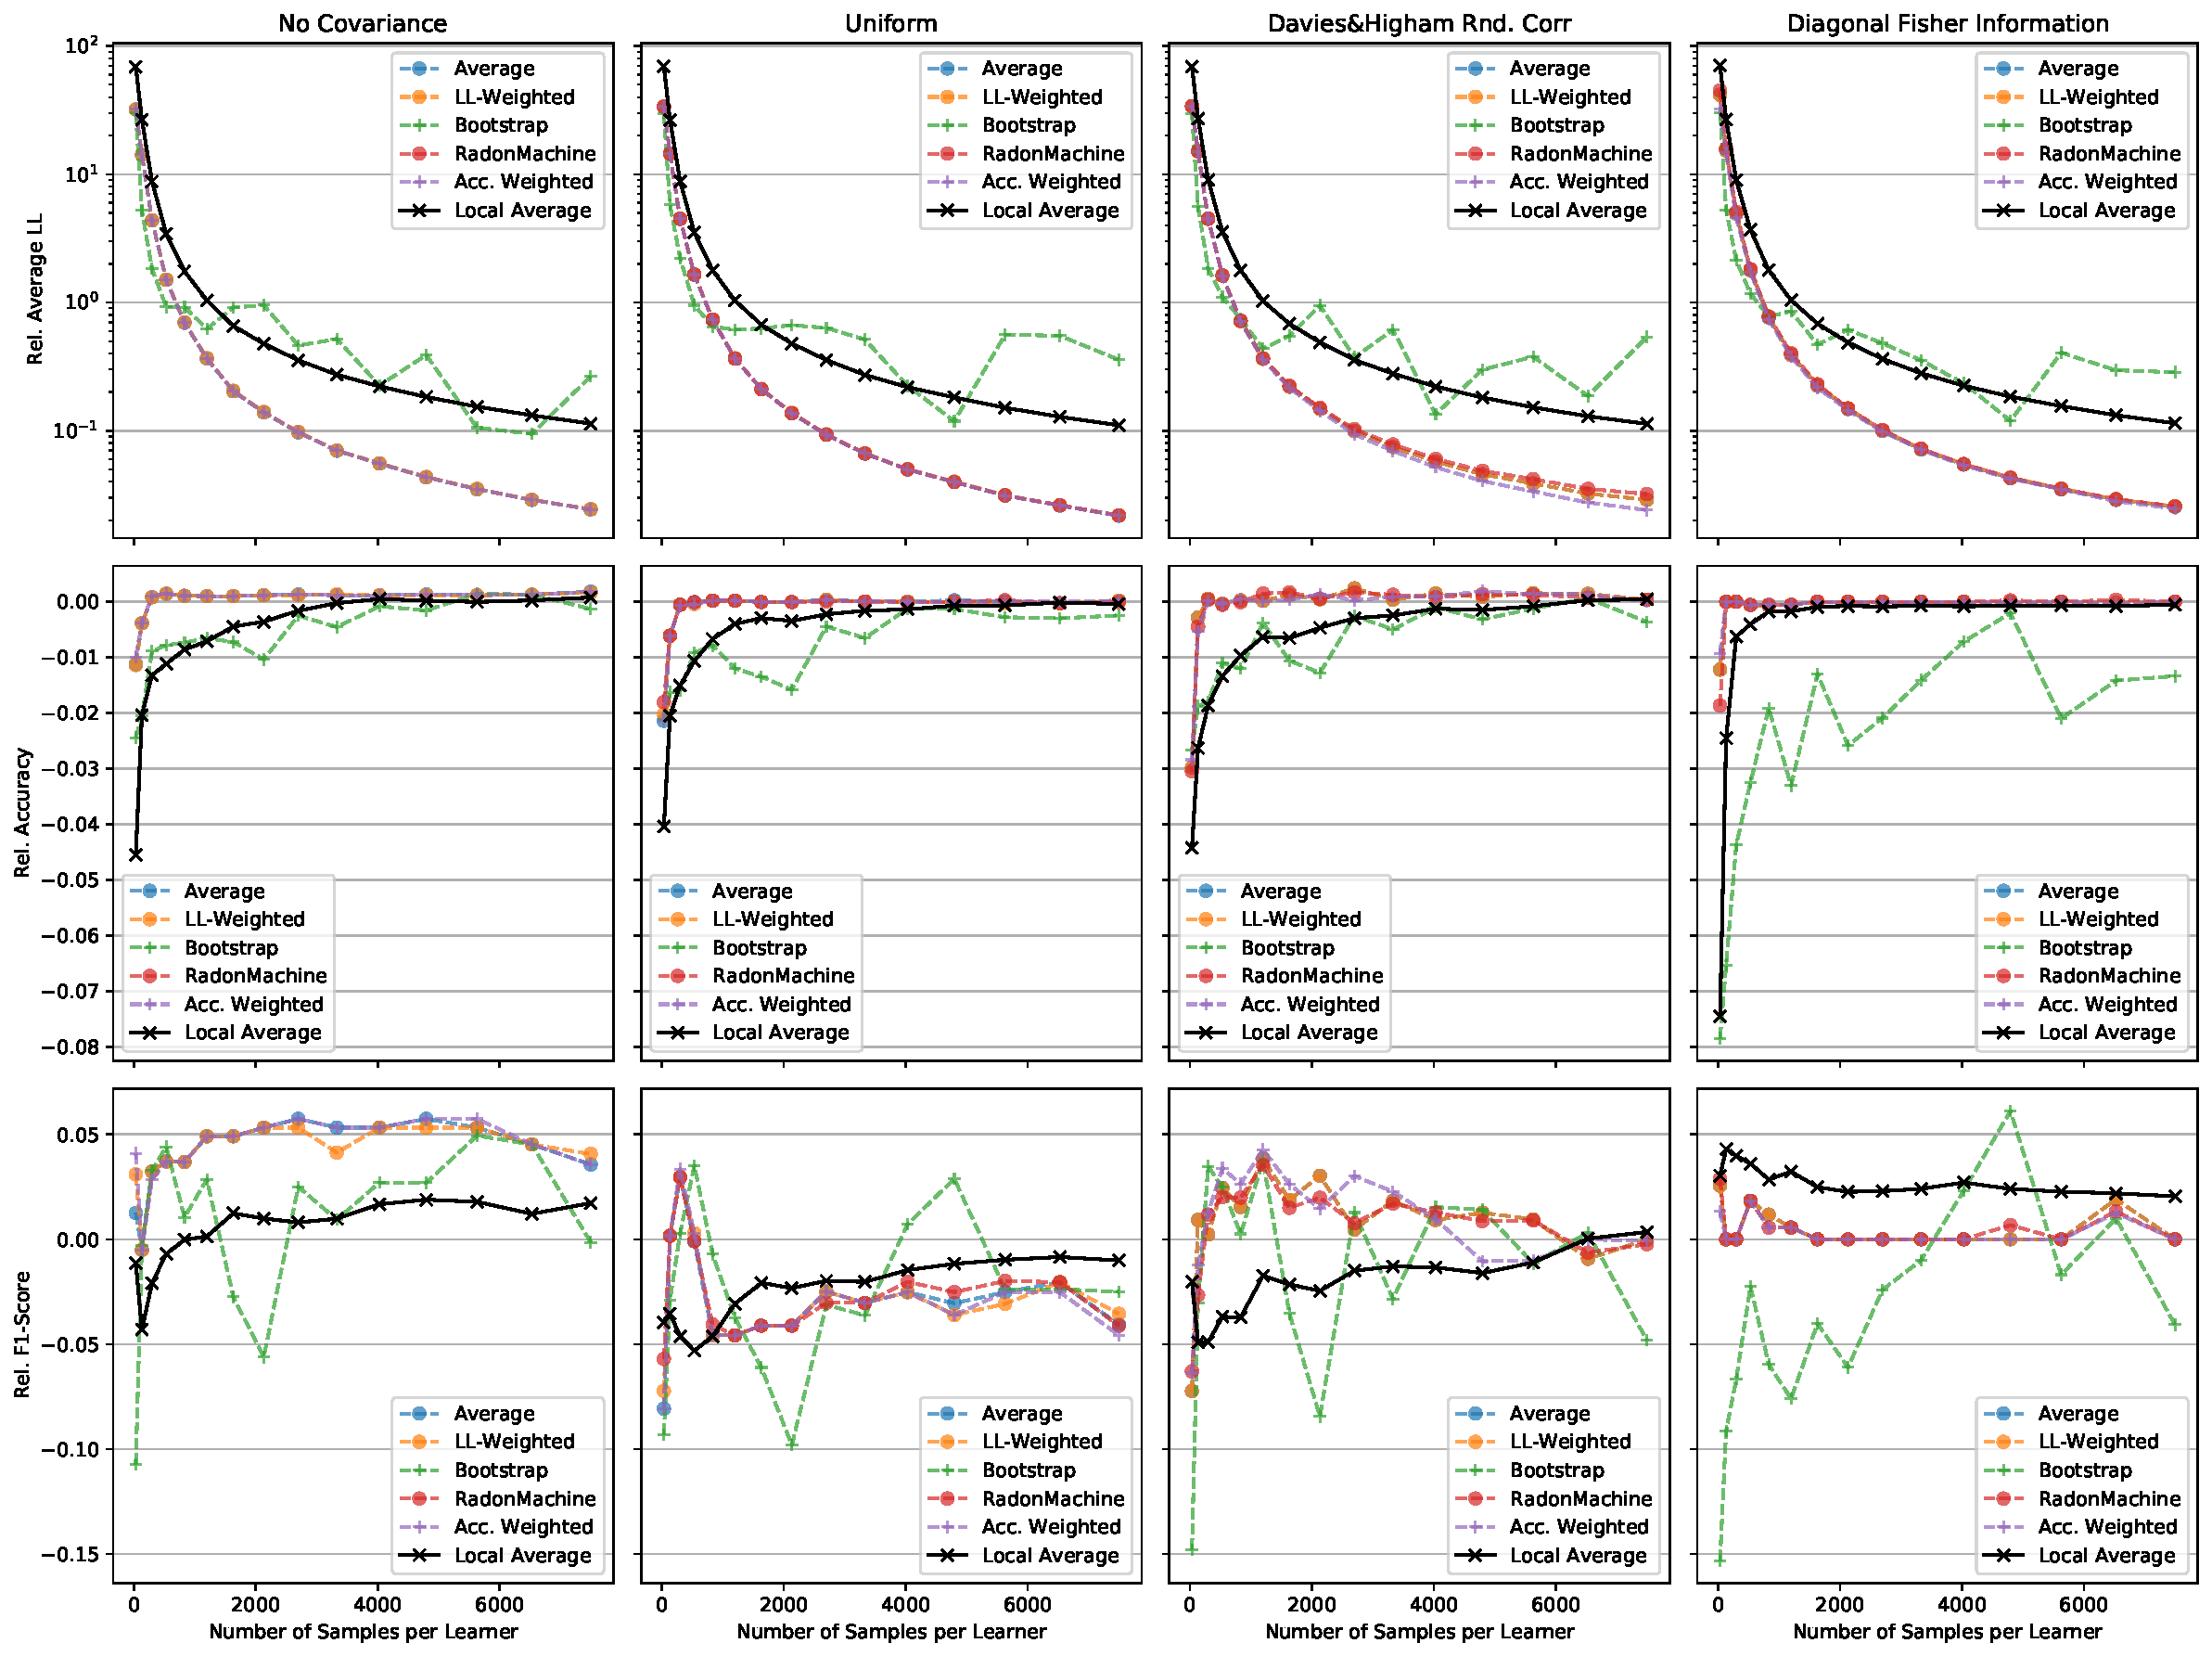
\includegraphics[height=\dimexpr \textheight - 4\baselineskip\relax]{kapitel/figures/susy_None_0.05_neg_relative.pdf}
        \caption[Susy without regularization and $\epsilon=0.05$]{Experimental results on the Susy data set for $k=10$ distributed learners. Each plot represents a combination of metric and covariance matrix used for sampling. Values on the x-Axis are the number of samples available on each learner. The top row shows the relative negative average log likelihood $\ell(\tilde{\vect{\theta}}; \mathcal{D}) - \ell(\hat{\vect{\theta}}; \mathcal{D})$ for each aggregate. Second and third row show accuracy and F1-score relative to the baseline on the test set.}
        \label{fig:analysis5}
    \end{figure}
    \end{landscape}
    \begin{landscape}
        \begin{figure}
            \centering
            \textbf{Susy, l2 regularization, Bound $\epsilon=0.1$}\par\medskip
            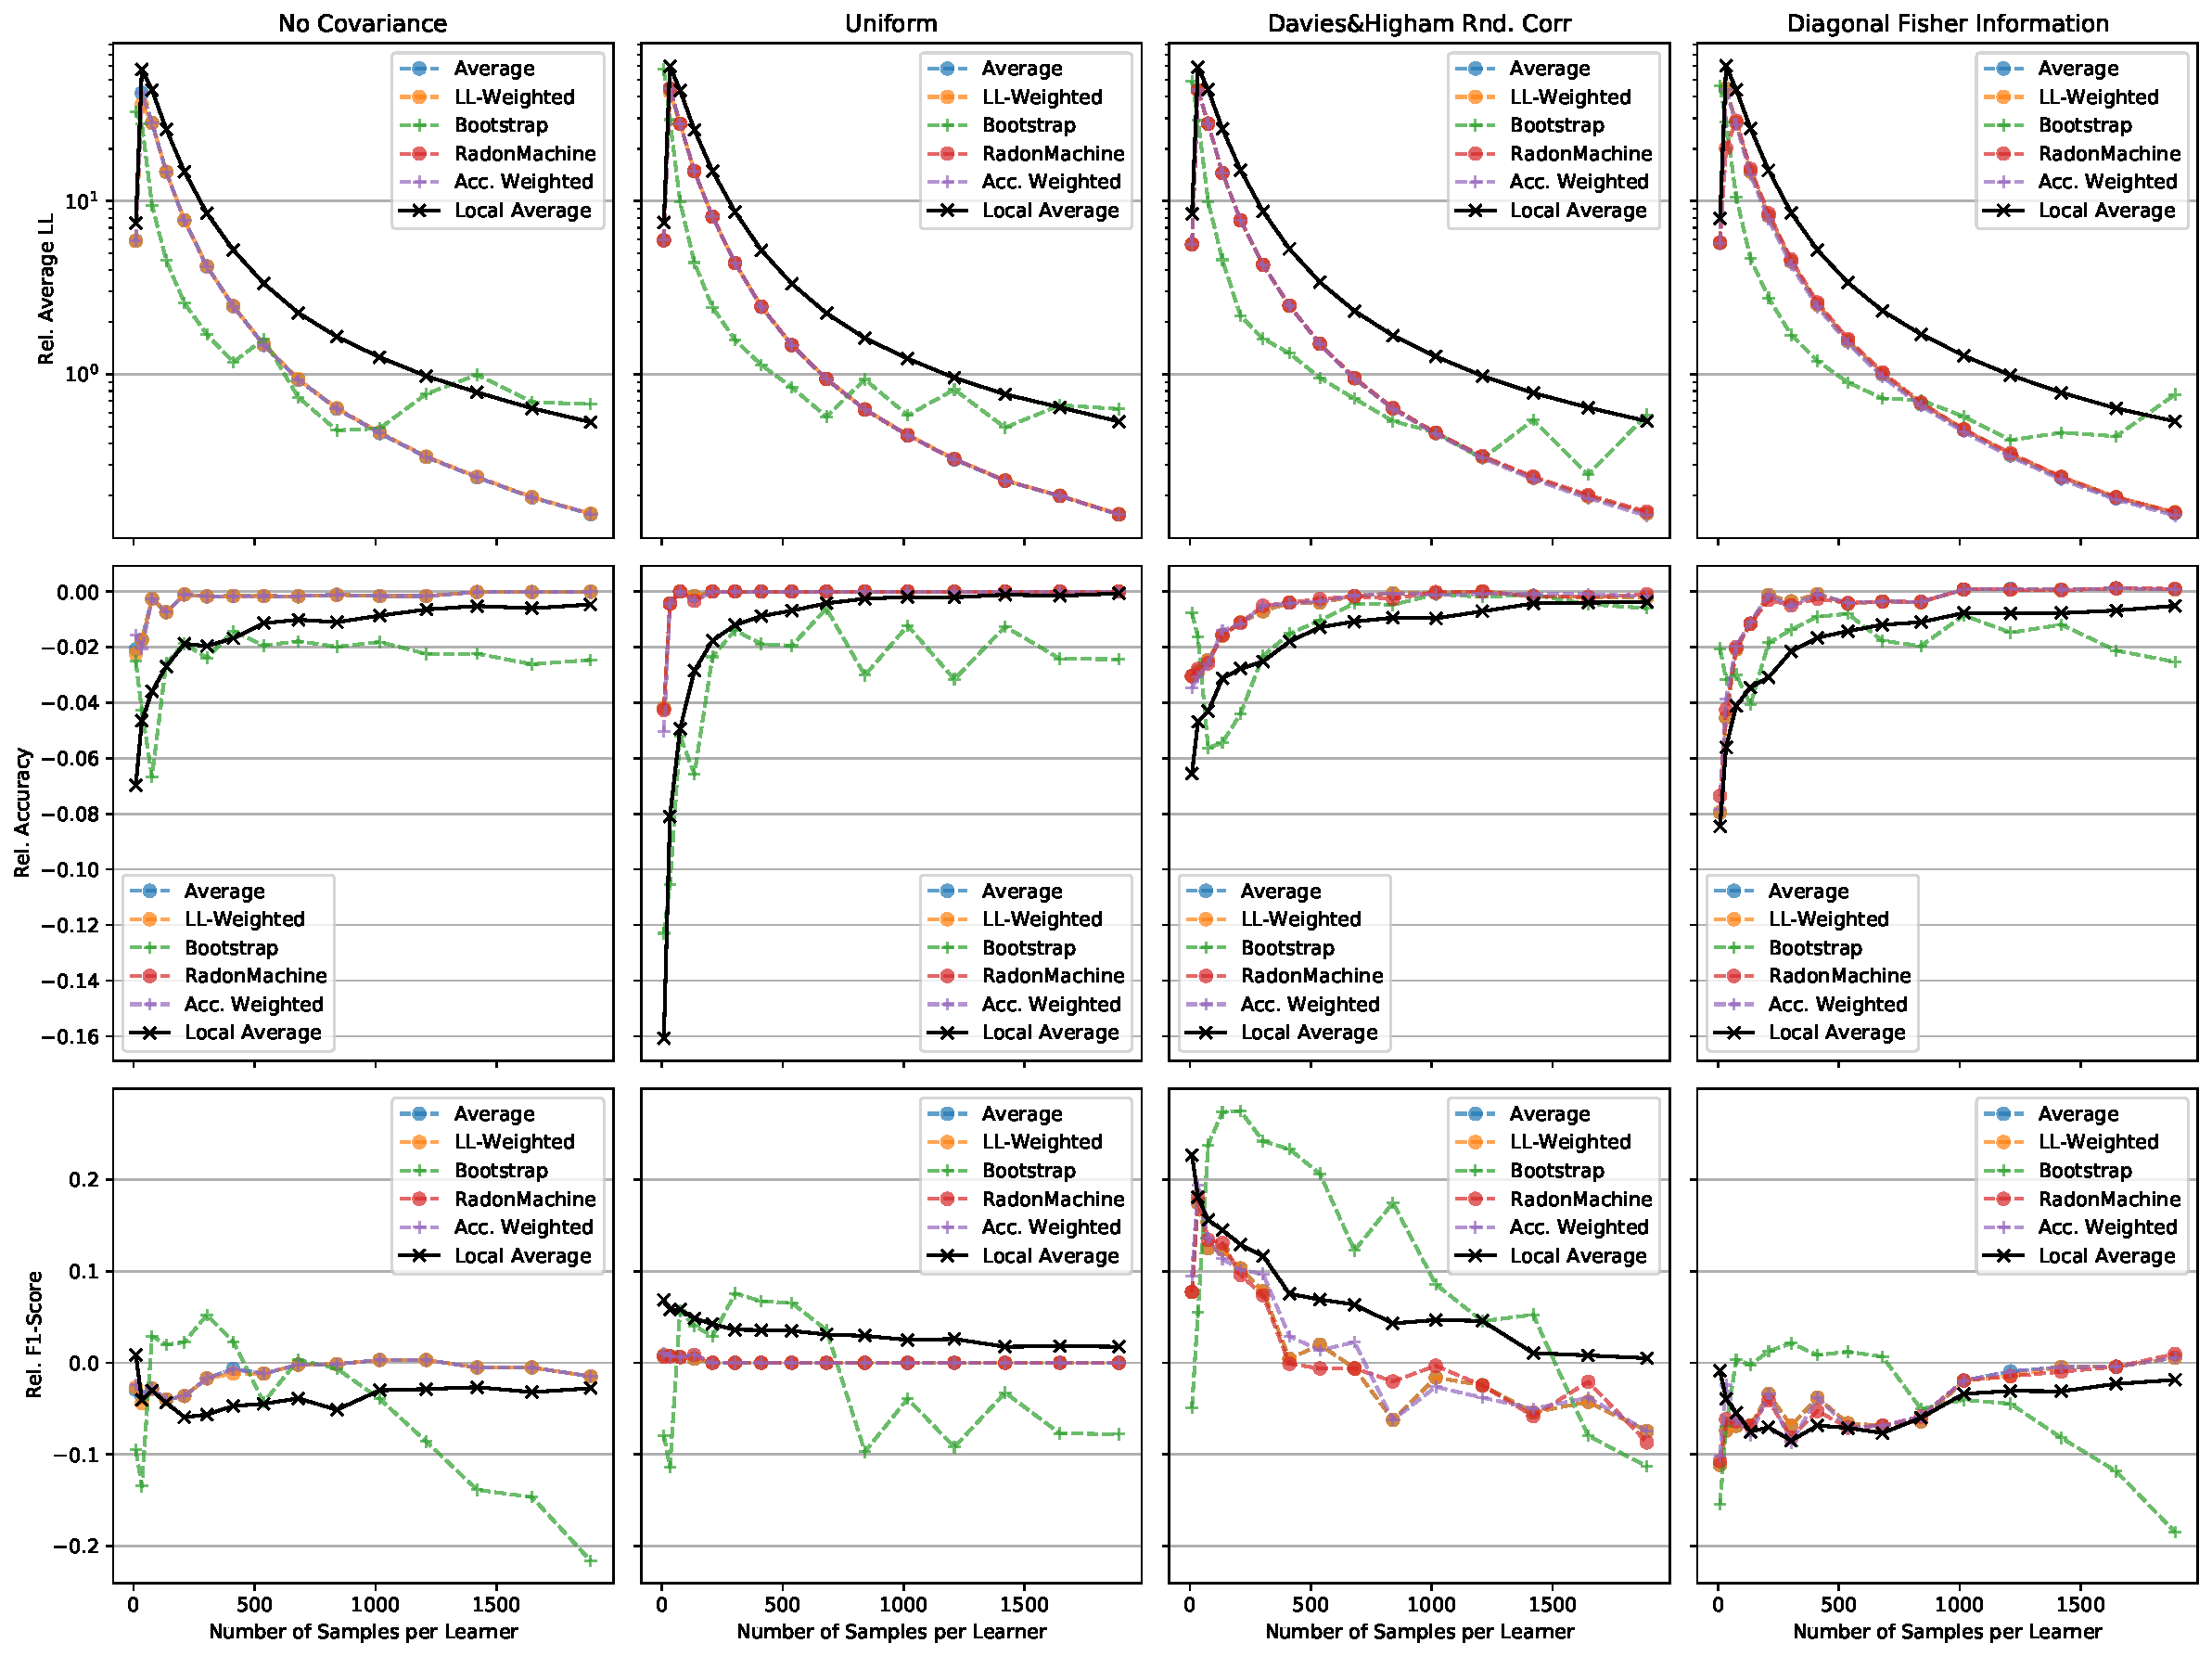
\includegraphics[height=\dimexpr \textheight - 4\baselineskip\relax]{kapitel/figures/susy_l2_0.1_neg_relative.pdf}
            \caption[Susy plots with l2 regularization and $\epsilon=0.1$]{Experimental results on the Susy data set for $k=10$ distributed learners. Each plot represents a combination of metric and covariance matrix used for sampling. Values on the x-Axis are the number of samples available on each learner. The top row shows the relative negative average log likelihood $\ell(\tilde{\vect{\theta}}; \mathcal{D}) - \ell(\hat{\vect{\theta}}; \mathcal{D})$ for each aggregate. Second and third row show accuracy and F1-score relative to the baseline on the test set.}
            \label{fig:analysis6}
        \end{figure}
    \end{landscape}

\begin{landscape}
    \begin{figure}
        \centering
        \textbf{Covertype, No regularization, Bound $\epsilon=0.1$}\par\medskip
        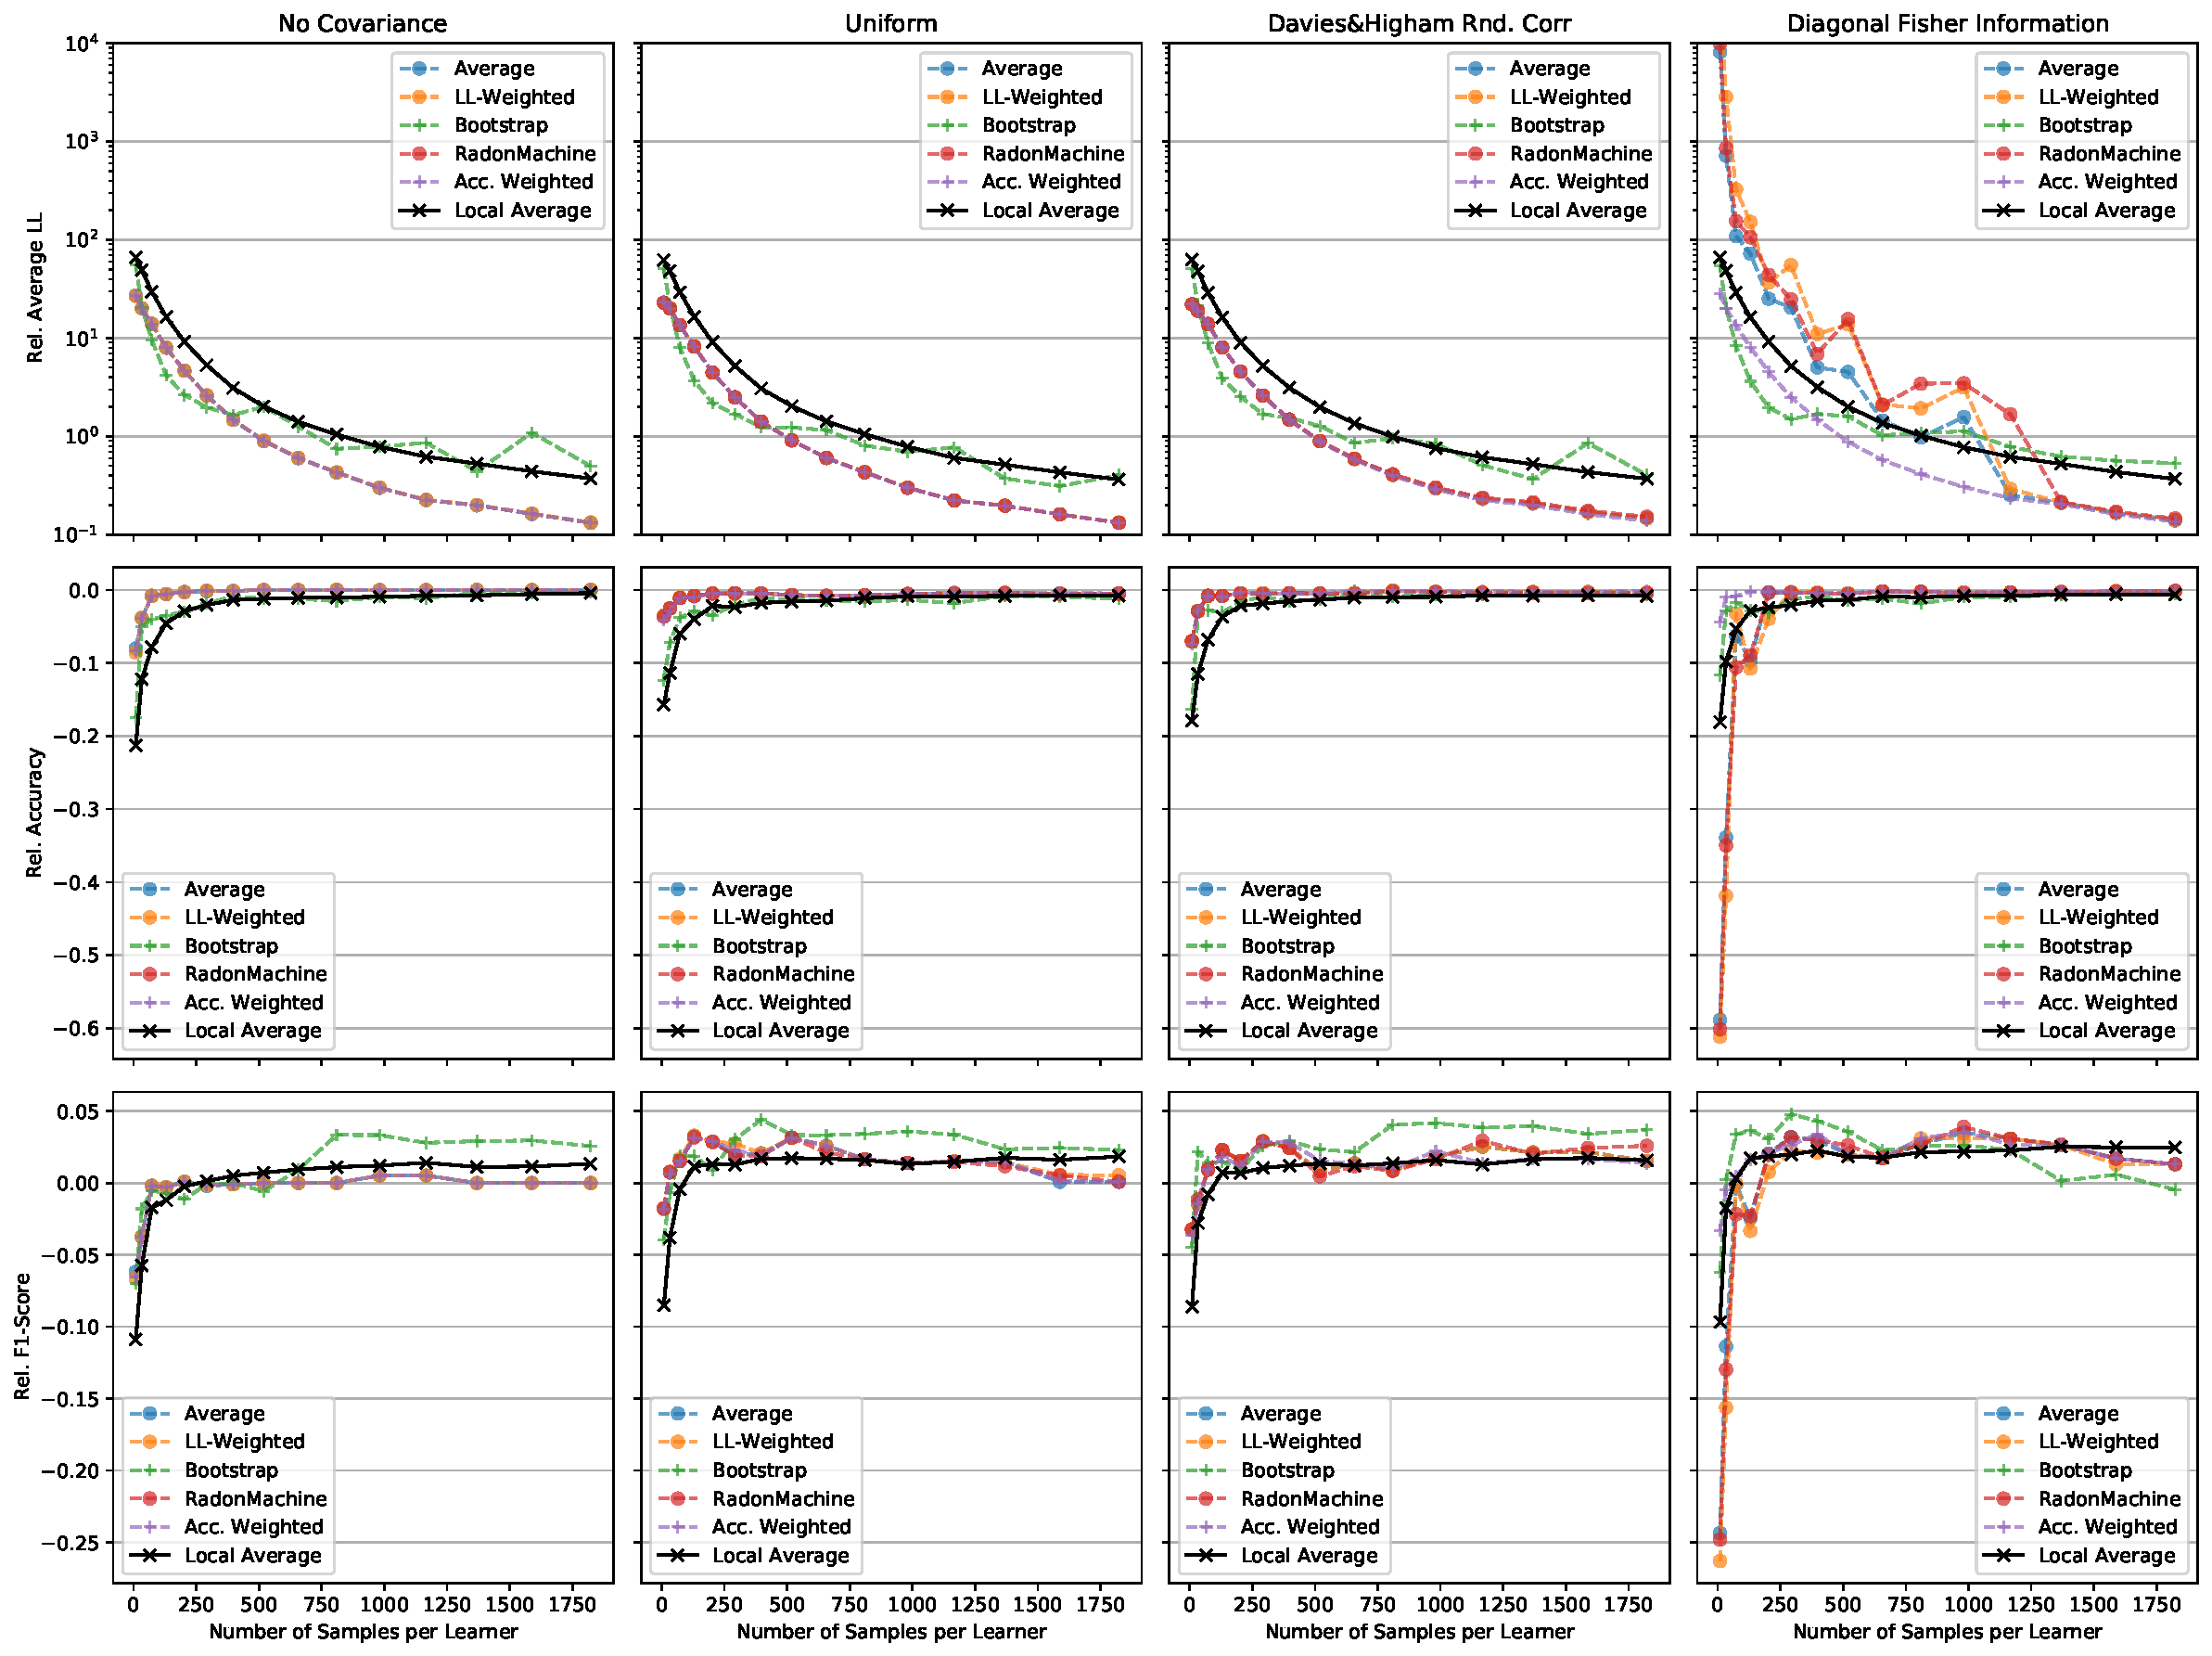
\includegraphics[height=\dimexpr \textheight - 4\baselineskip\relax]{kapitel/figures/covertype_None_0.1_neg_relative.pdf}
        \caption[Covertype plots without regularization and $\epsilon=0.1$]{Experimental results on the Covertype data set for $k=10$ distributed learners. Each plot represents a combination of metric and covariance matrix used for sampling. Values on the x-Axis are the number of samples available on each learner.The top row shows the relative negative average log likelihood $\ell(\tilde{\vect{\theta}}; \mathcal{D}) - \ell(\hat{\vect{\theta}}; \mathcal{D})$ for each aggregate. Second and third row show accuracy and F1-score relative to the baseline on the test set.}
        \label{fig:analysis7}
    \end{figure}
    \end{landscape}
    \begin{landscape}
    \begin{figure}
        \centering
        \textbf{Covertype, No regularization, Bound $\epsilon=0.05$}\par\medskip
        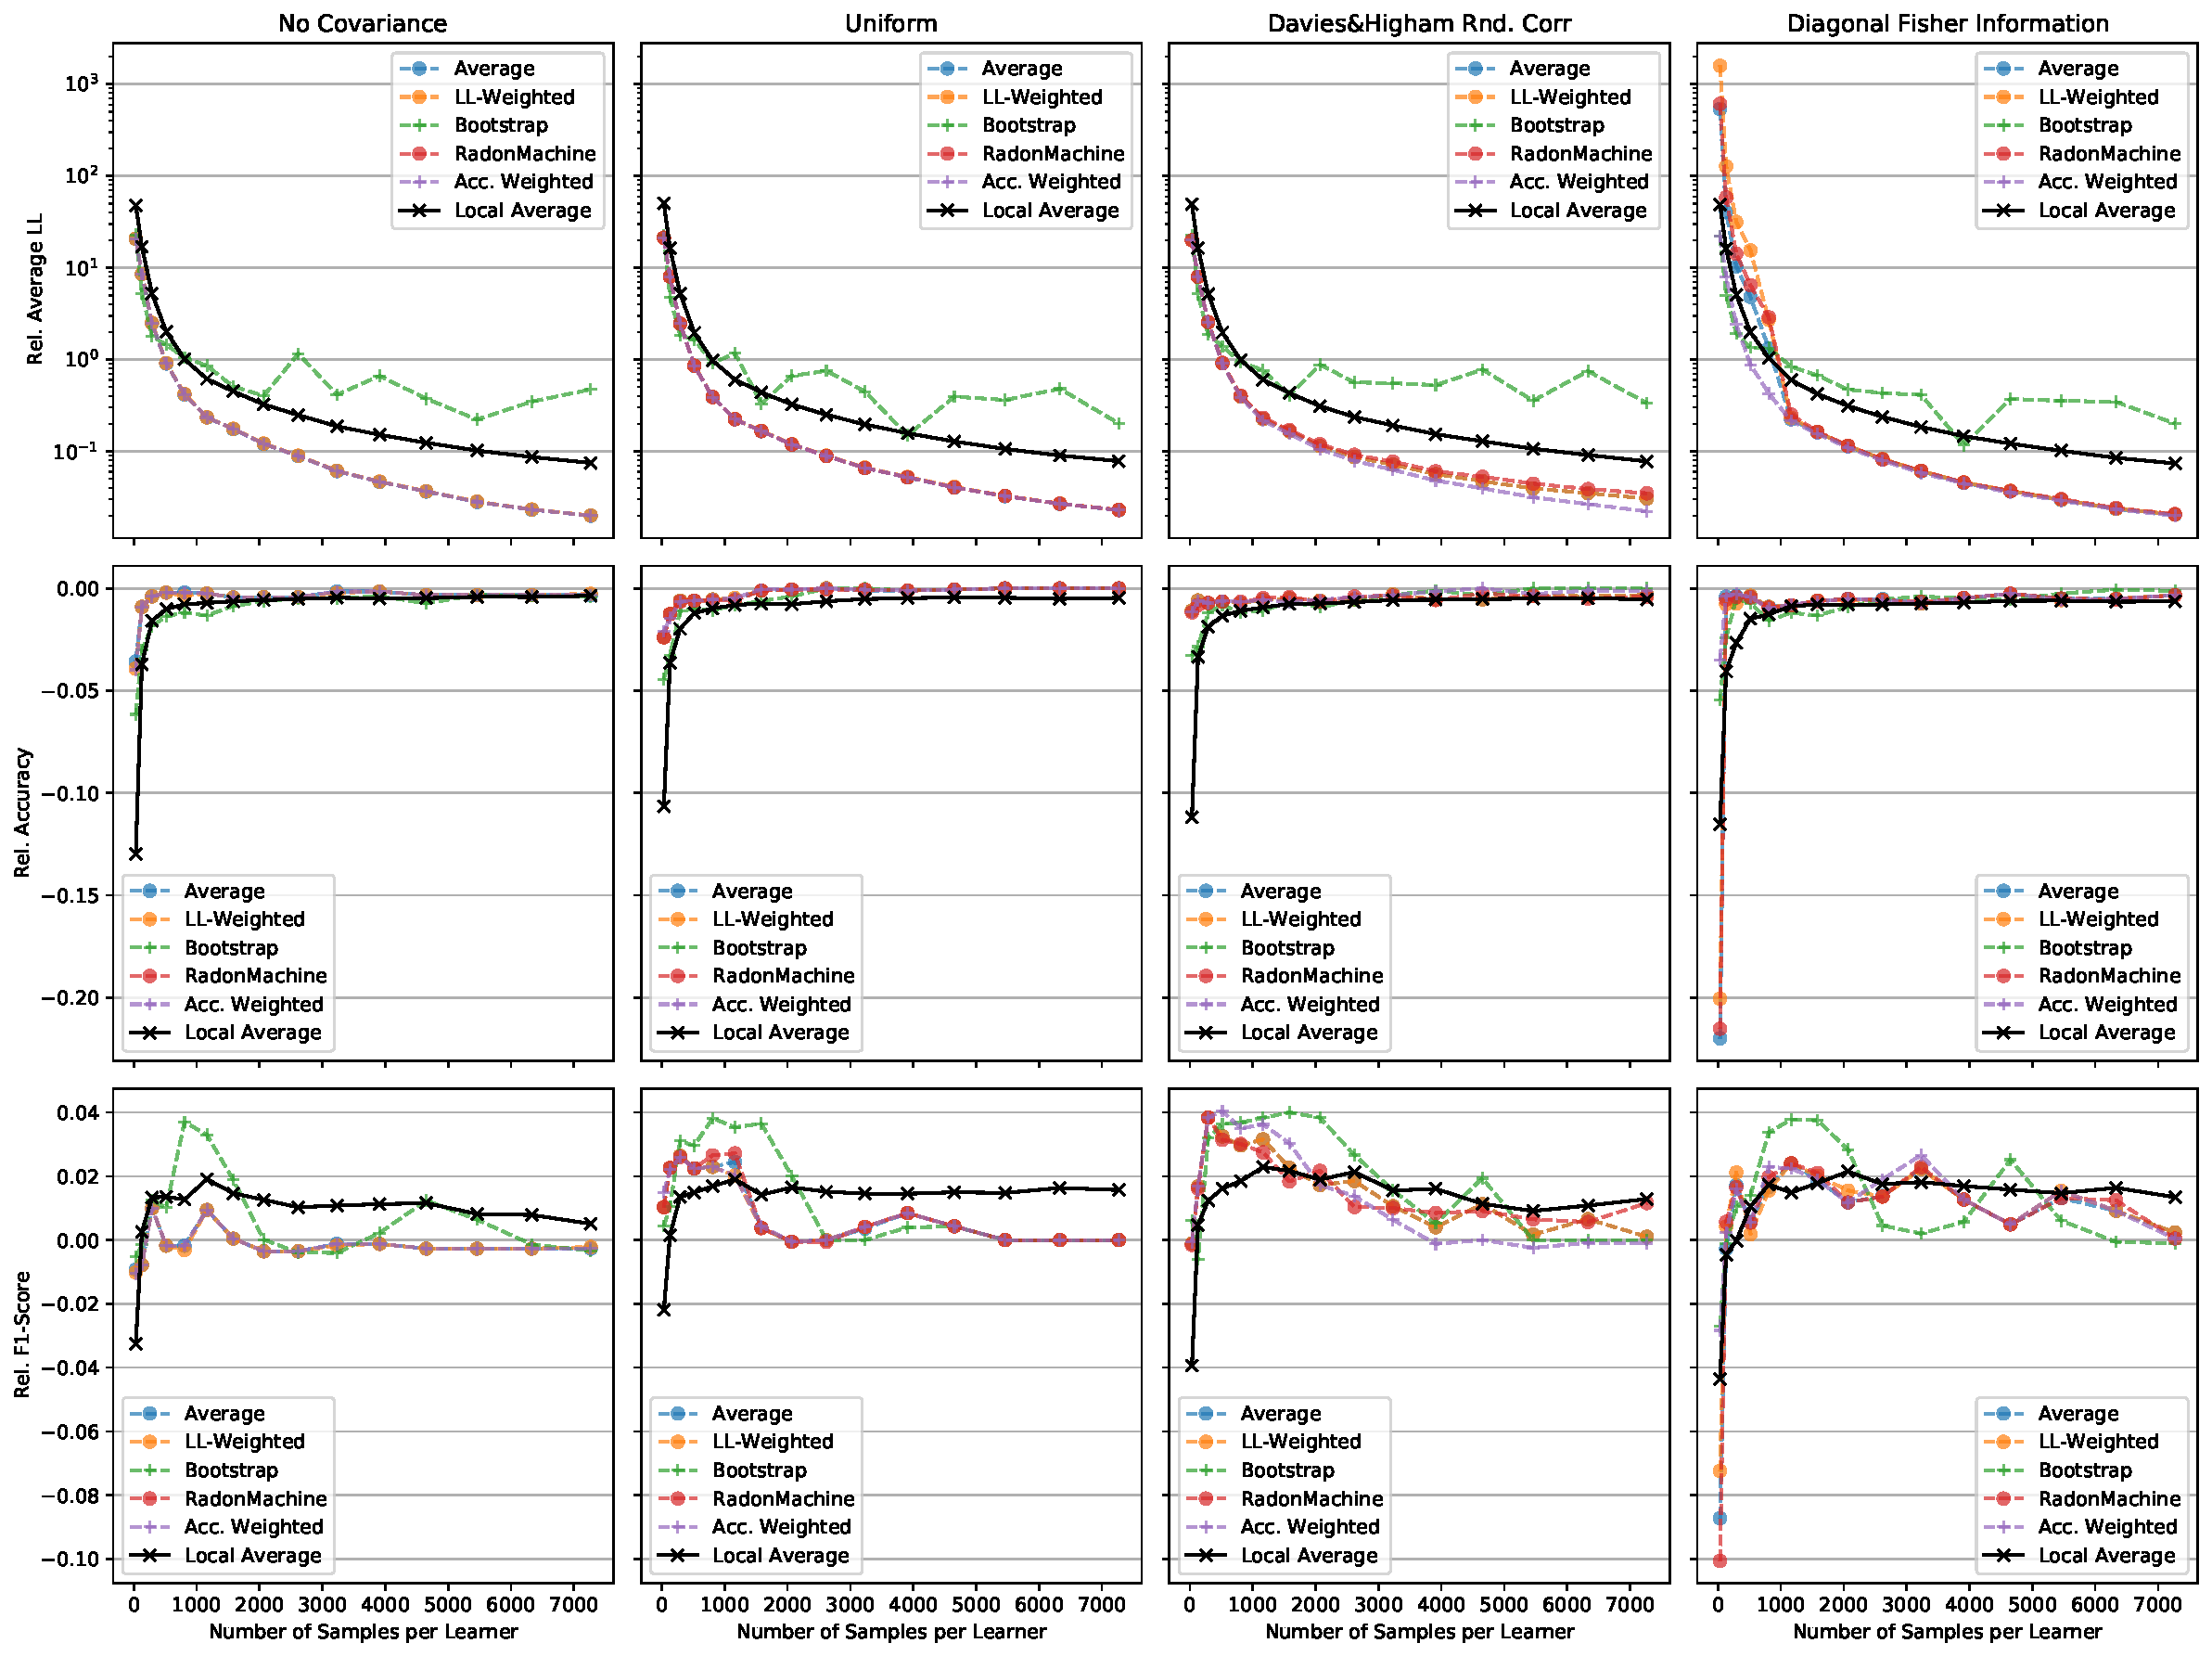
\includegraphics[height=\dimexpr \textheight - 4\baselineskip\relax]{kapitel/figures/covertype_None_0.05_neg_relative.pdf}
        \caption[Covertype without regularization and $\epsilon=0.05$]{Experimental results on the Covertype data set for $k=10$ distributed learners. Each plot represents a combination of metric and covariance matrix used for sampling. Values on the x-Axis are the number of samples available on each learner. The top row shows the relative negative average log likelihood $\ell(\tilde{\vect{\theta}}; \mathcal{D}) - \ell(\hat{\vect{\theta}}; \mathcal{D})$ for each aggregate. Second and third row show accuracy and F1-score relative to the baseline on the test set.}
        \label{fig:analysis8}
    \end{figure}
    \end{landscape}
    \begin{landscape}
        \begin{figure}
            \centering
            \textbf{Covertype, l2 regularization, Bound $\epsilon=0.1$}\par\medskip
            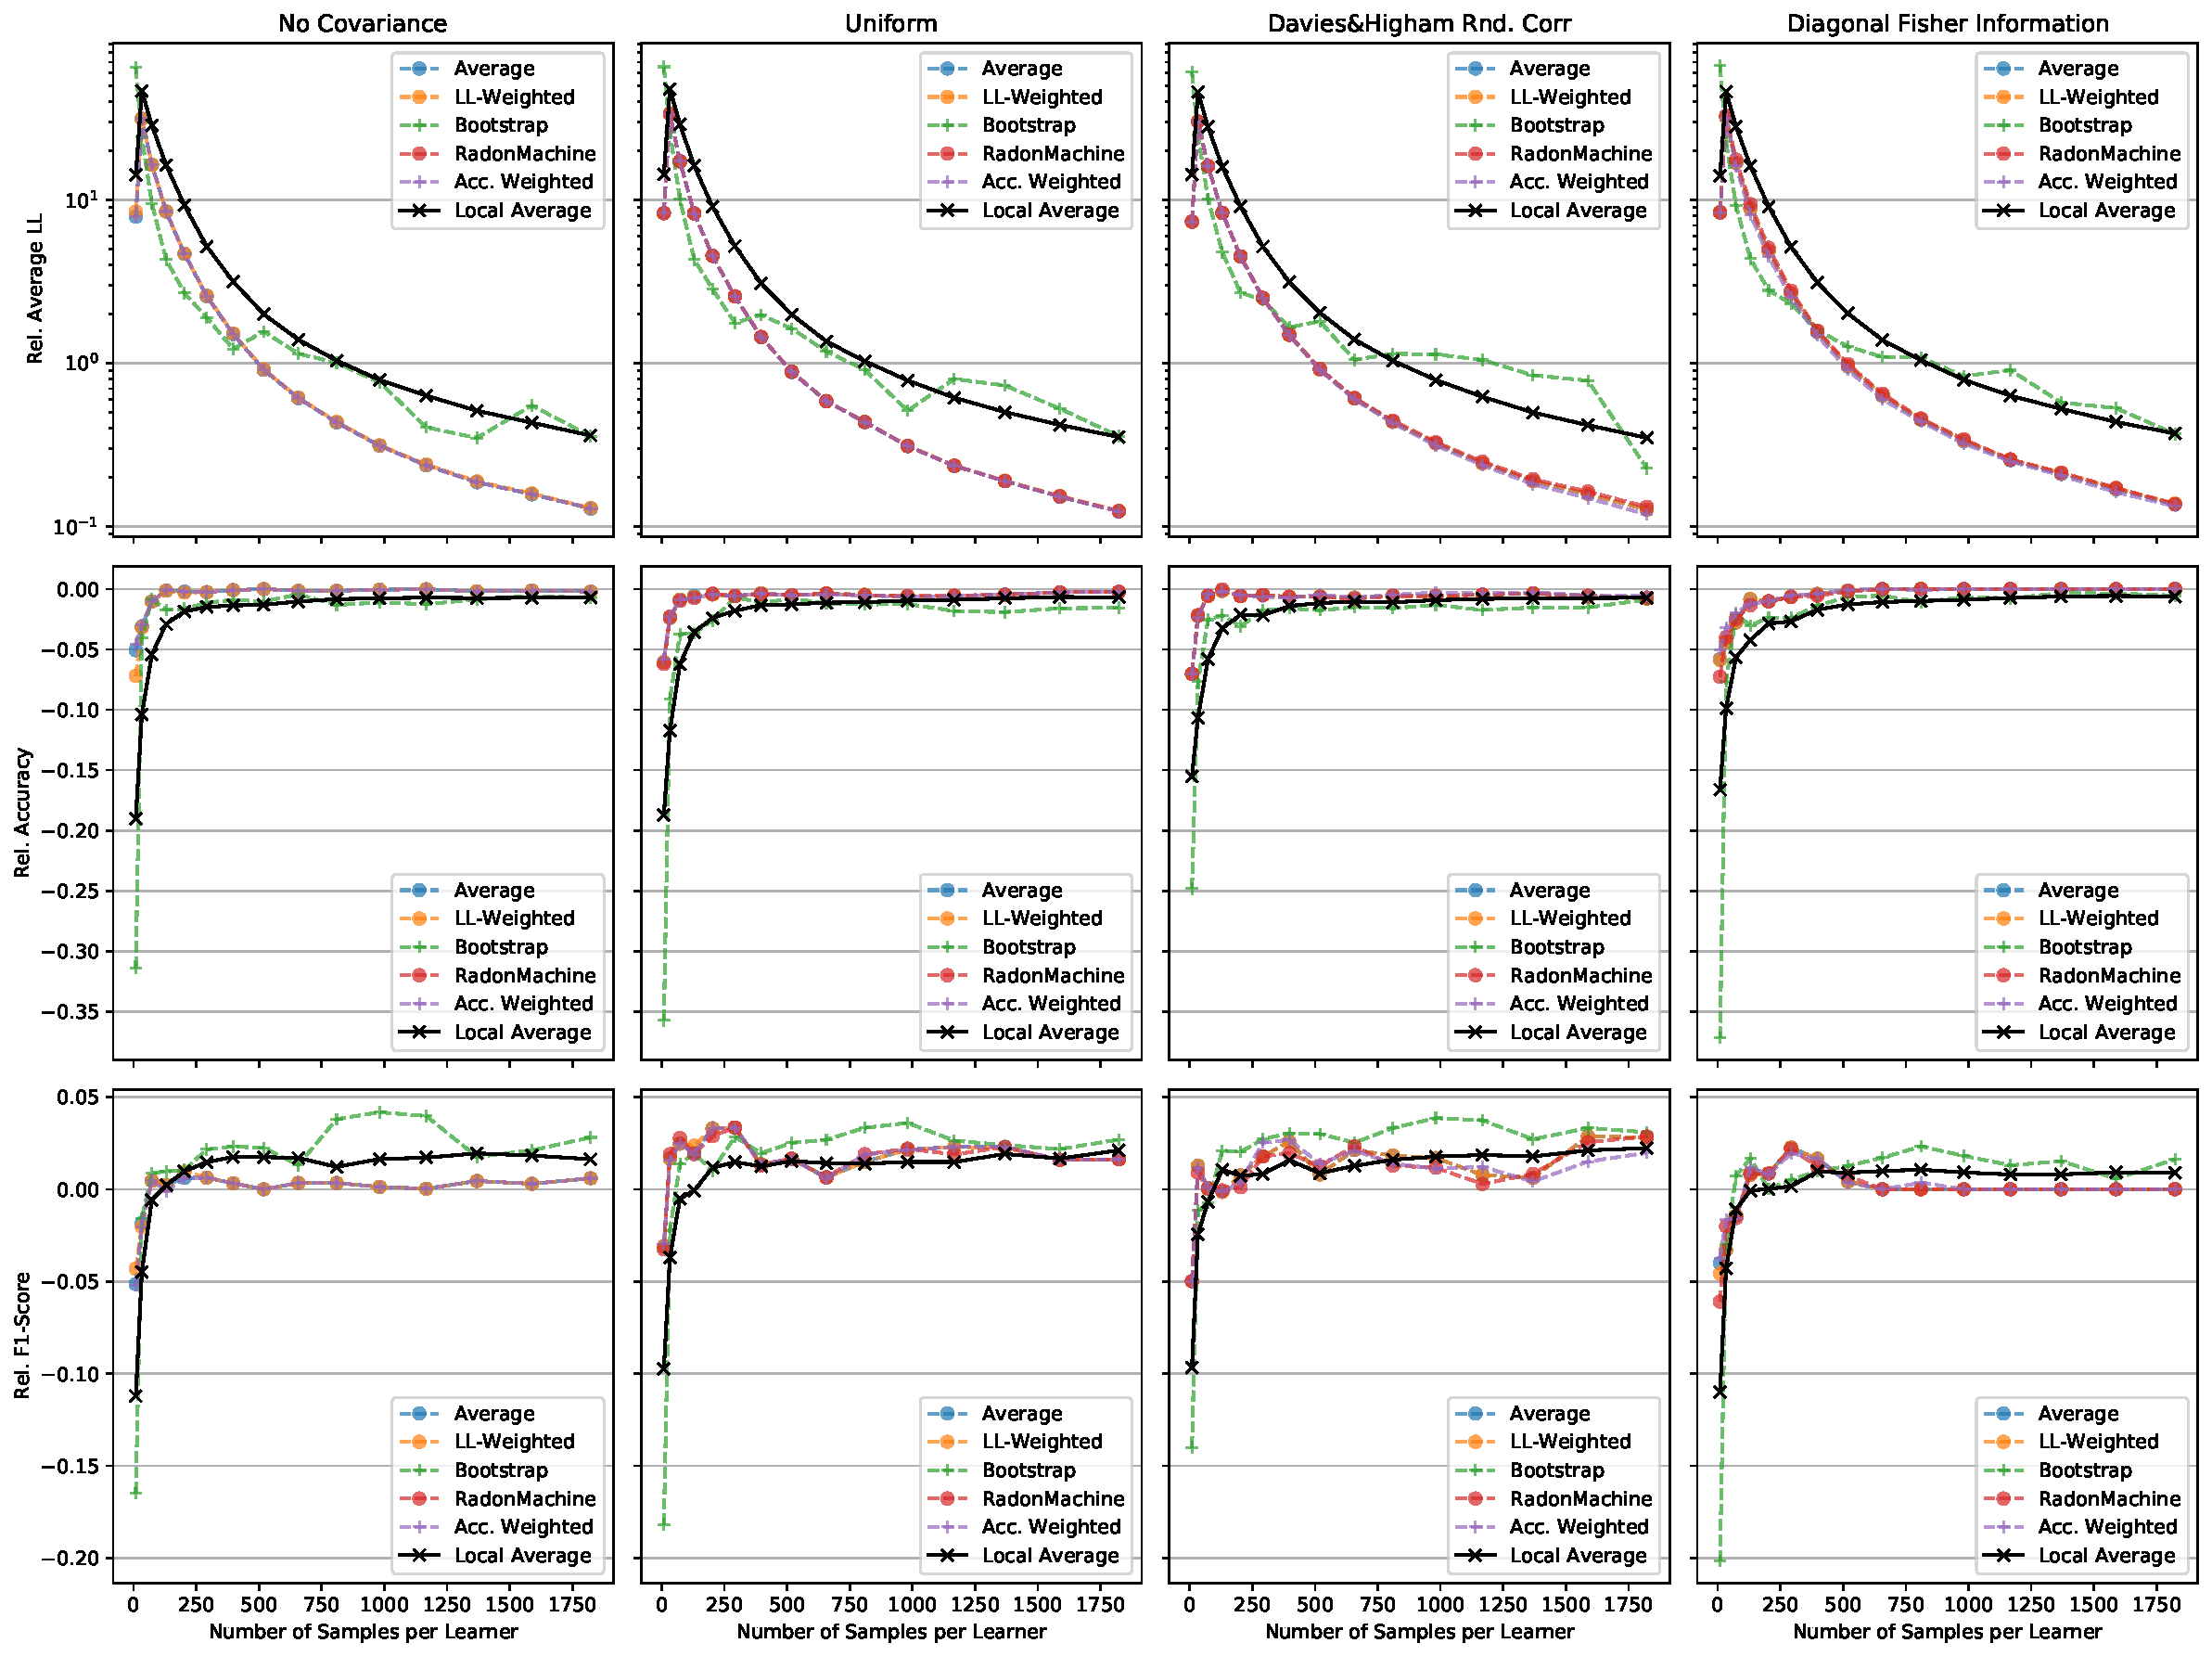
\includegraphics[height=\dimexpr \textheight - 4\baselineskip\relax]{kapitel/figures/covertype_l2_0.1_neg_relative.pdf}
            \caption[Covertype plots with l2 regularization and $\epsilon=0.1$]{Experimental results on the Covertype data set for $k=10$ distributed learners. Each plot represents a combination of metric and covariance matrix used for sampling. Values on the x-Axis are the number of samples available on each learner. The top row shows the relative negative average log likelihood $\ell(\tilde{\vect{\theta}}; \mathcal{D}) - \ell(\hat{\vect{\theta}}; \mathcal{D})$ for each aggregate. Second and third row show accuracy and F1-score relative to the baseline on the test set.}
            \label{fig:analysis9}
        \end{figure}
    \end{landscape}

\begin{landscape}
    \begin{figure}
        \centering
        \textbf{Dota2, No regularization, Bound $\epsilon=0.1$}\par\medskip
        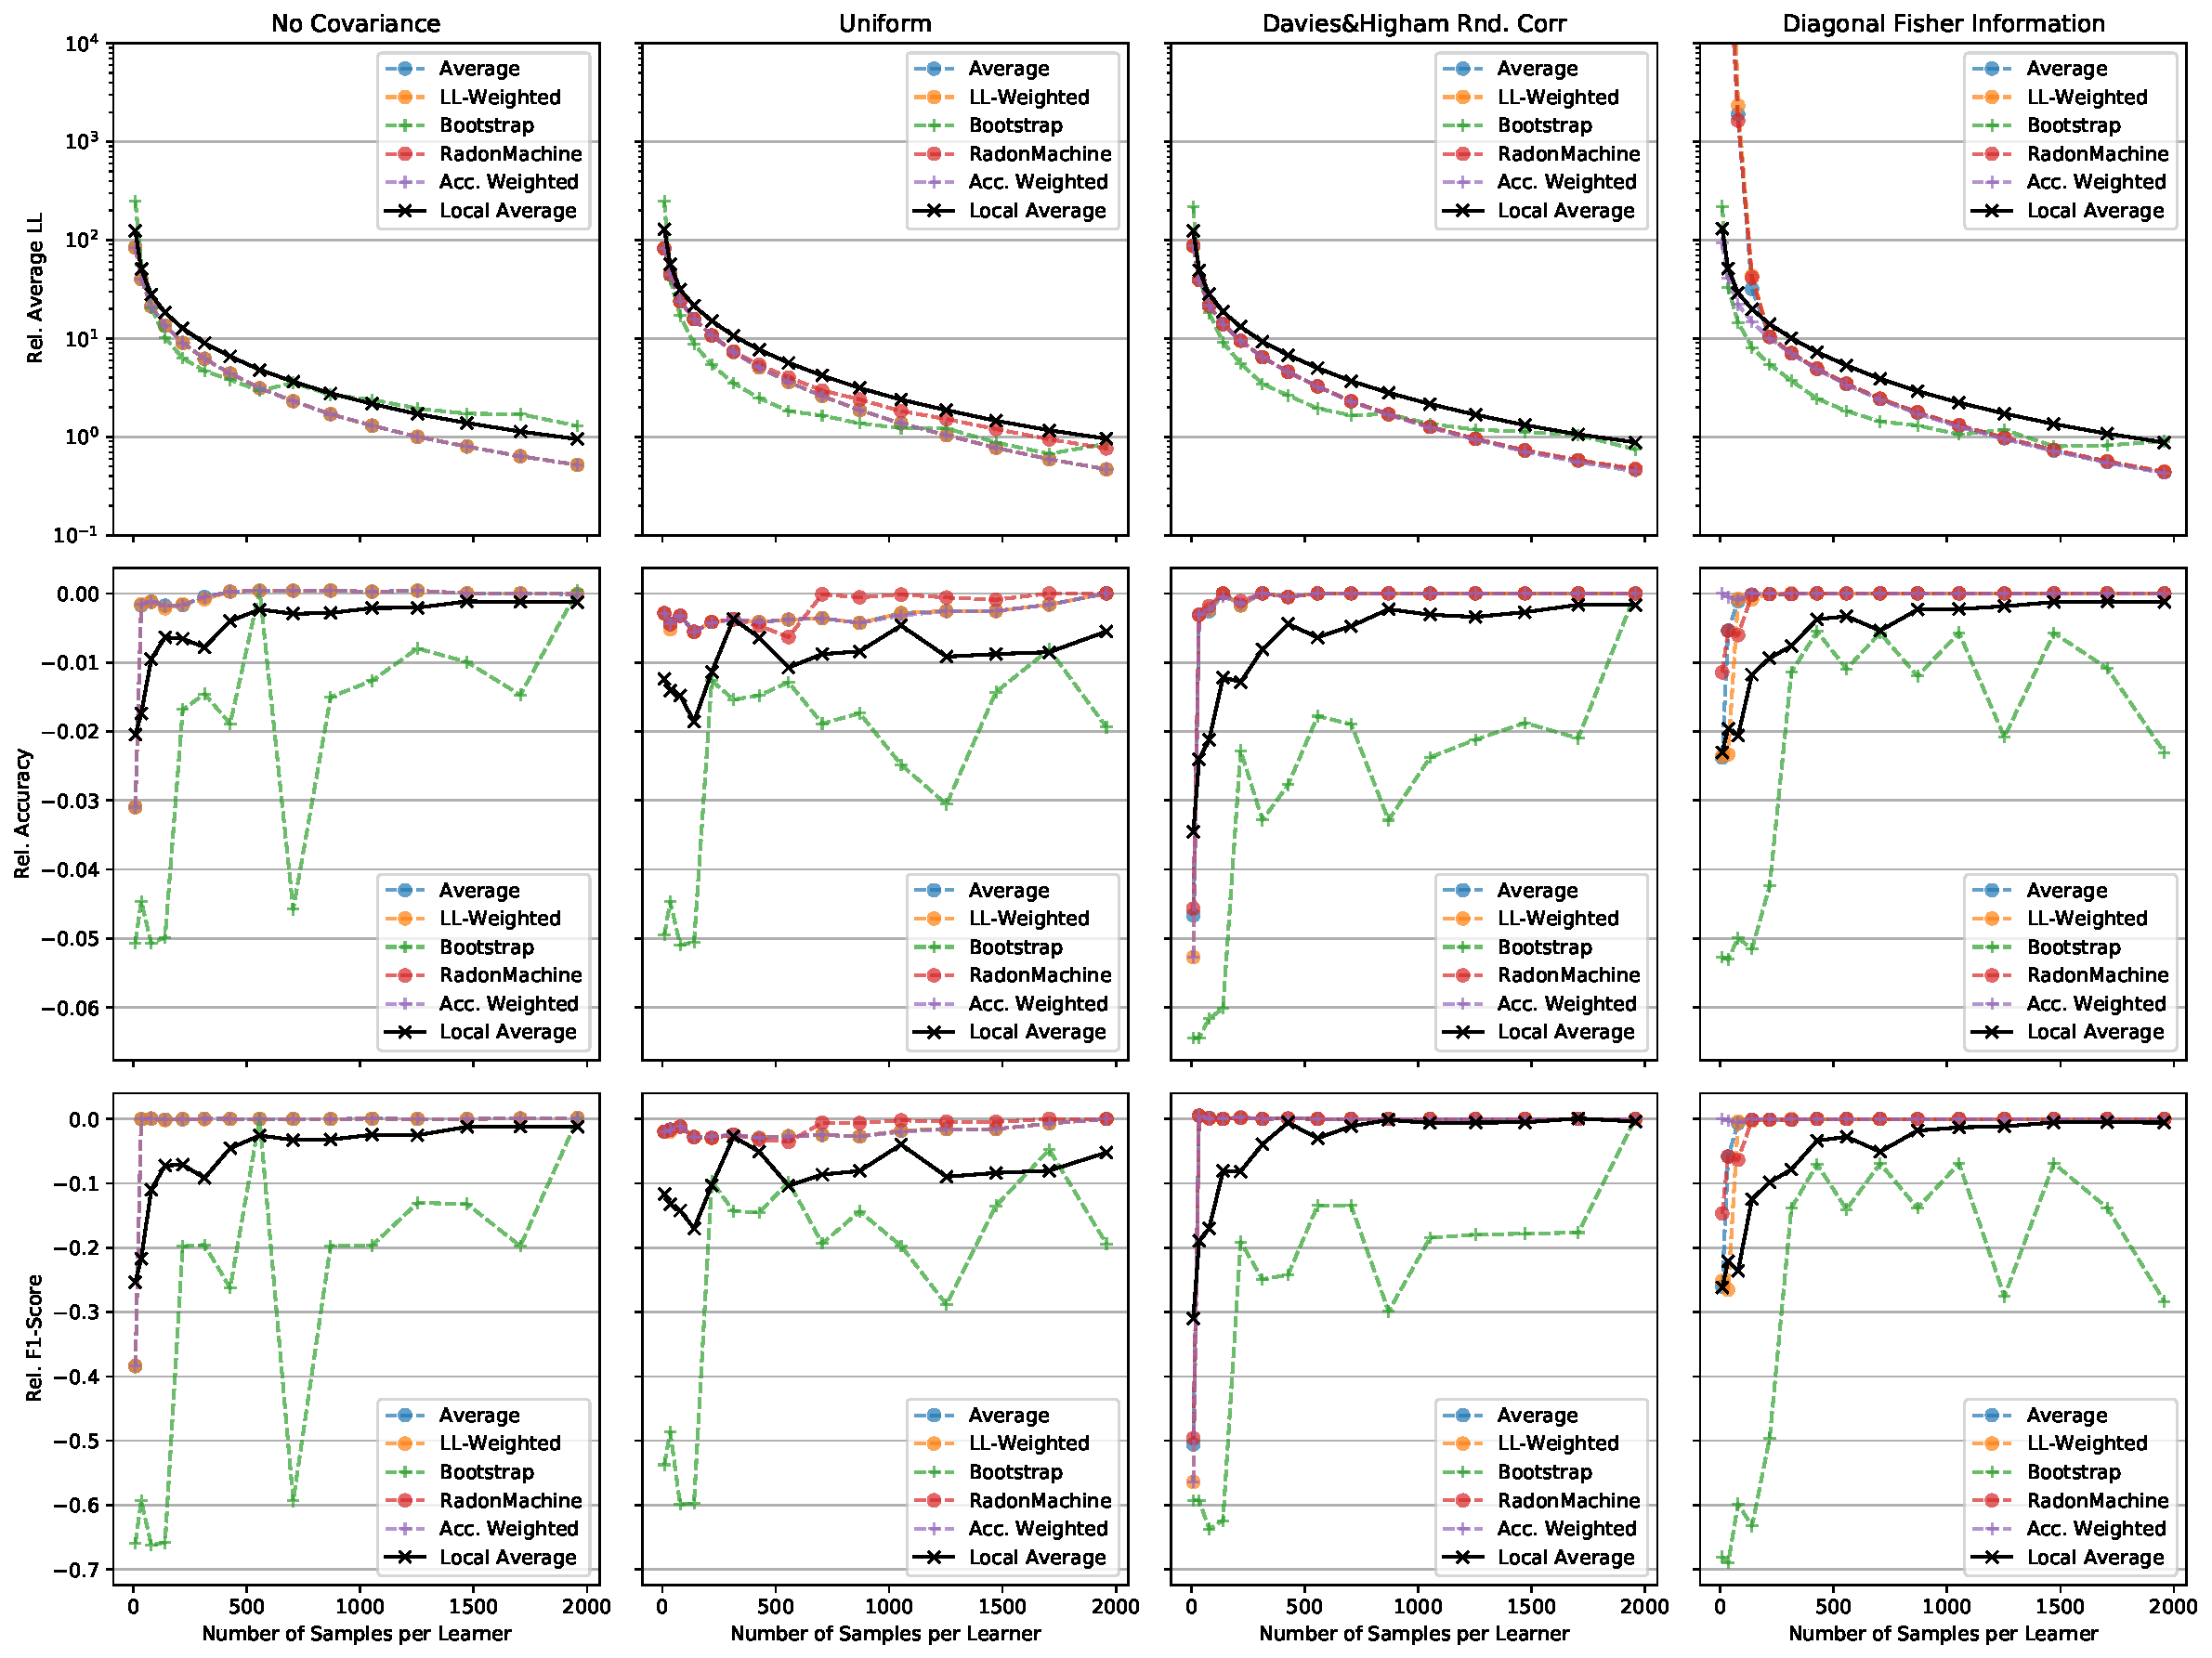
\includegraphics[height=\dimexpr \textheight - 4\baselineskip\relax]{kapitel/figures/dota2_None_0.1_neg_relative.pdf}
        \caption[Dota2 plots without regularization and $\epsilon=0.1$]{Experimental results on the Dota2 data set for $k=10$ distributed learners. Each plot represents a combination of metric and covariance matrix used for sampling. Values on the x-Axis are the number of samples available on each learner.The top row shows the relative negative average log likelihood $\ell(\tilde{\vect{\theta}}; \mathcal{D}) - \ell(\hat{\vect{\theta}}; \mathcal{D})$ for each aggregate. Second and third row show accuracy and F1-score relative to the baseline on the test set.}
        \label{fig:analysis10}
    \end{figure}
    \end{landscape}
    \begin{landscape}
    \begin{figure}
        \centering
        \textbf{Dota2, No regularization, Bound $\epsilon=0.05$}\par\medskip
        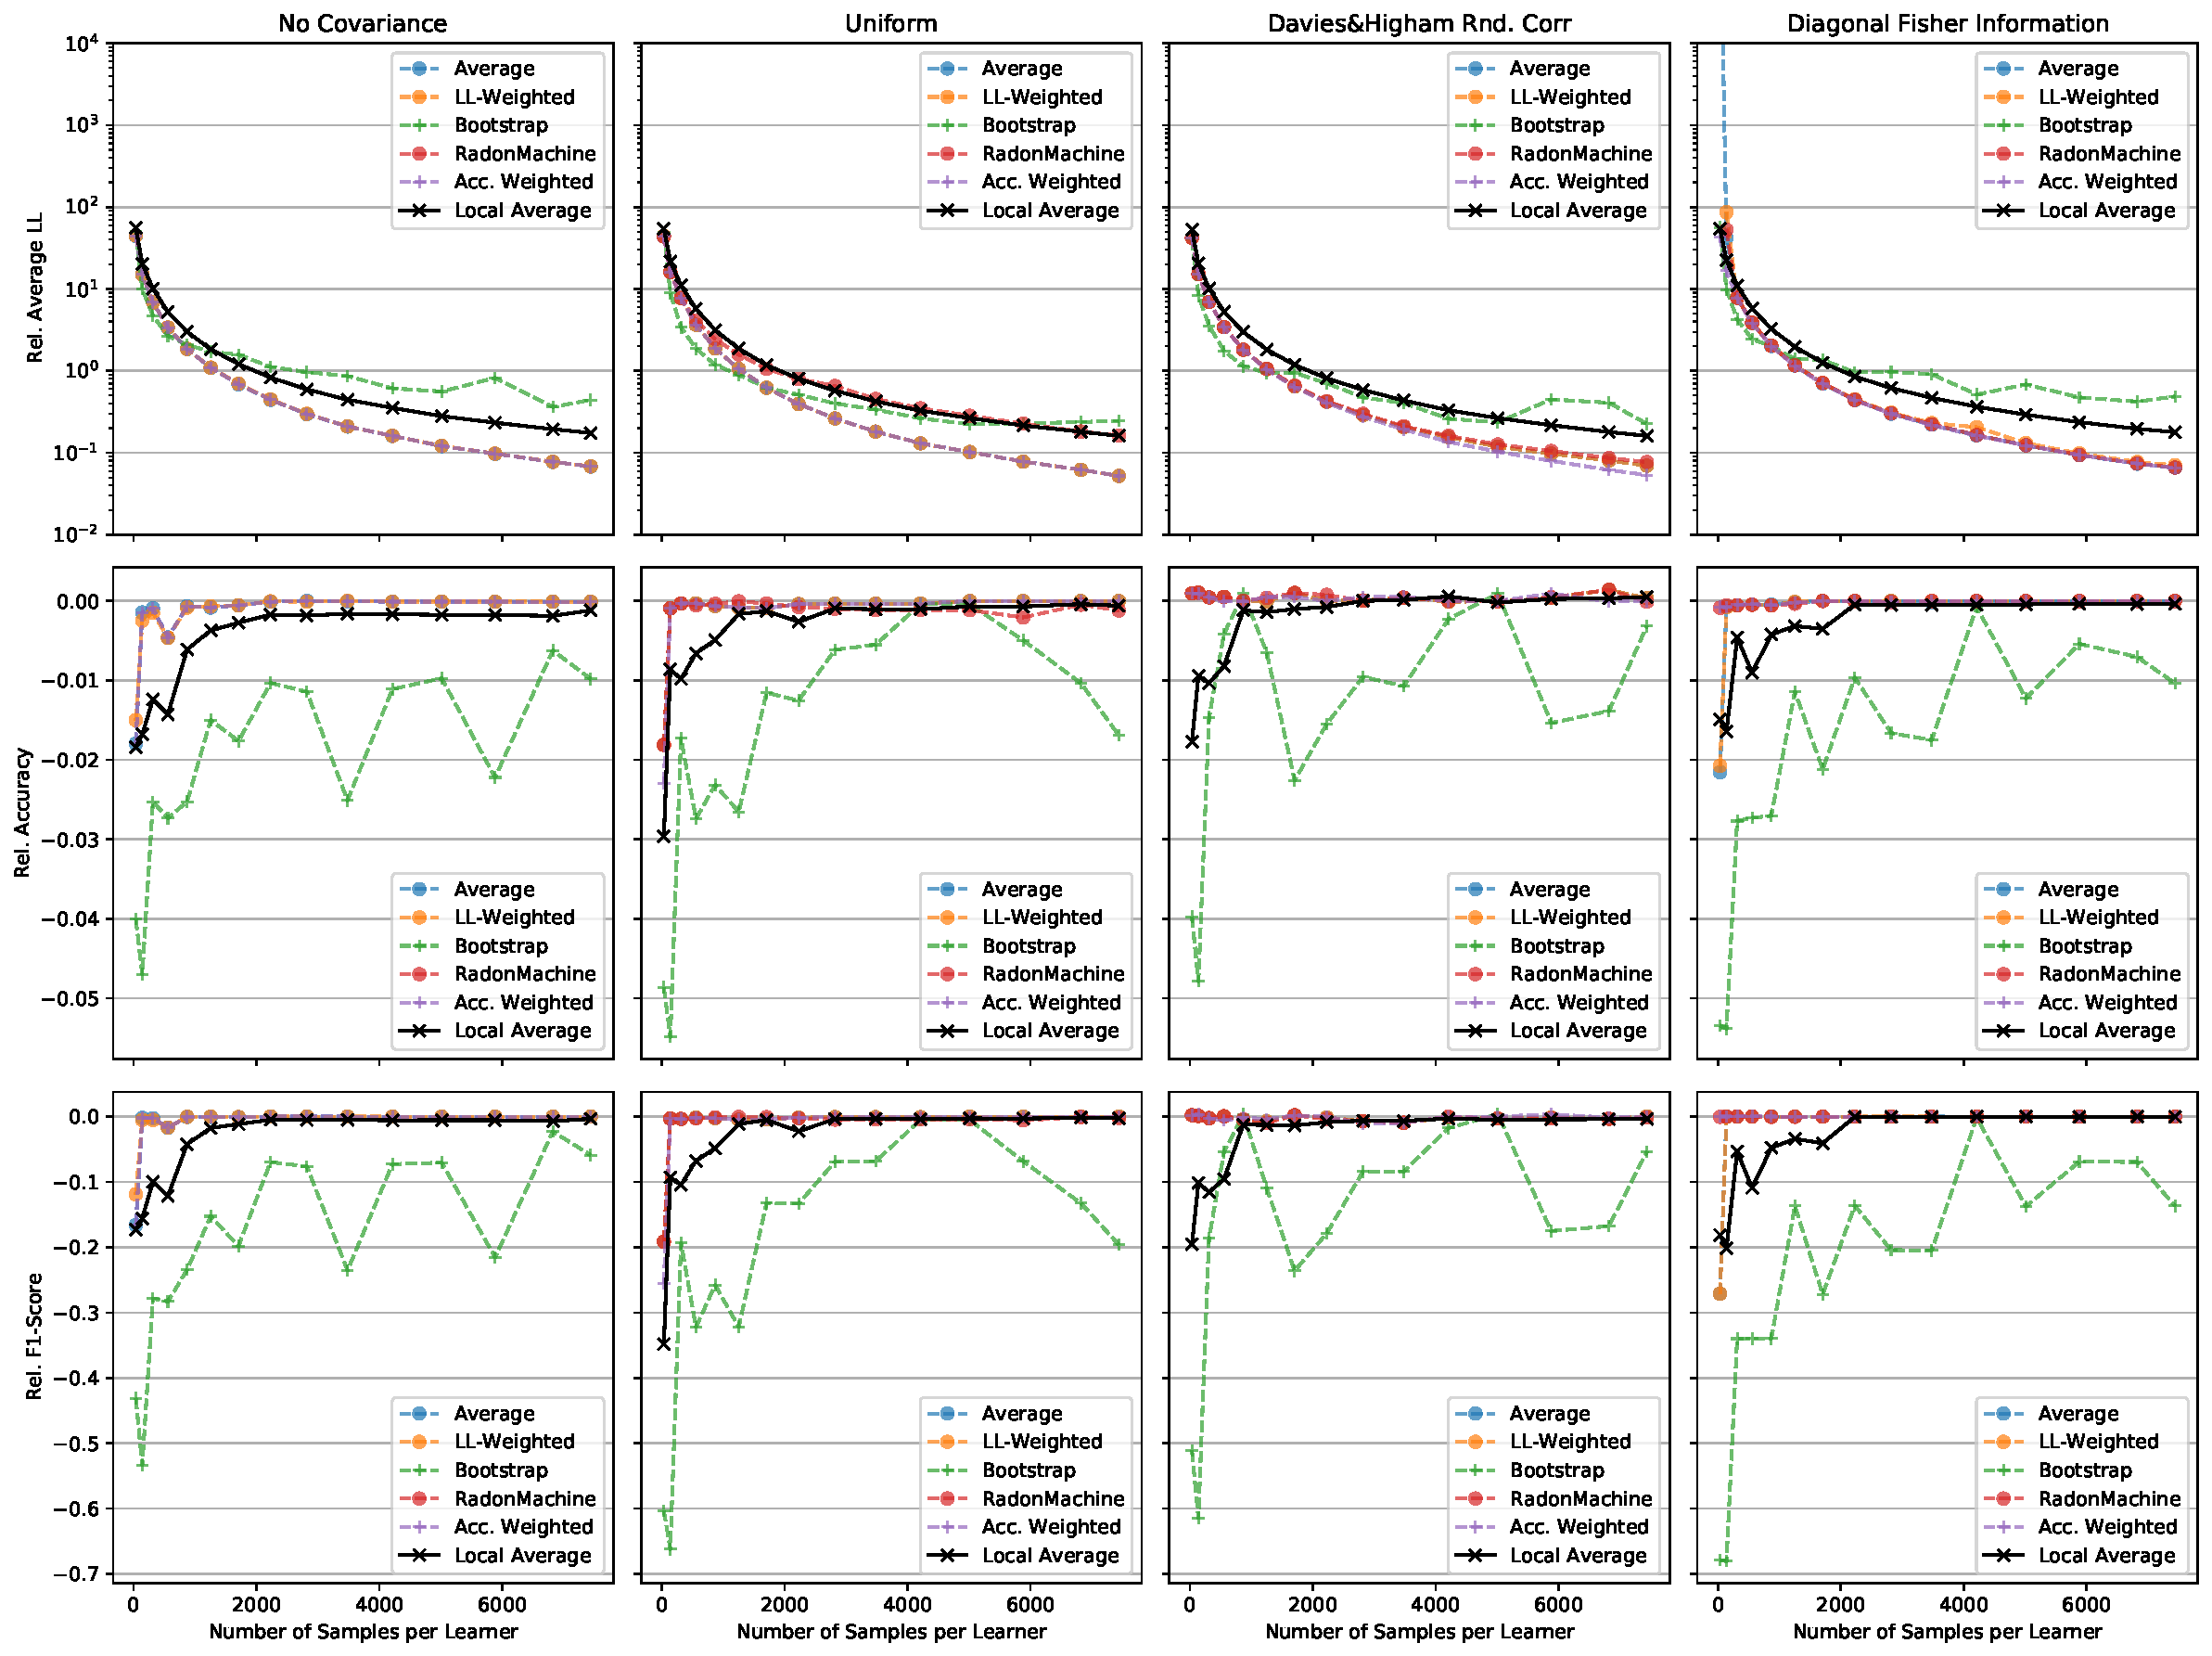
\includegraphics[height=\dimexpr \textheight - 4\baselineskip\relax]{kapitel/figures/dota2_None_0.05_neg_relative.pdf}
        \caption[Dota2 plots without regularization and $\epsilon=0.05$]{Experimental results on the Dota2 data set for $k=10$ distributed learners. Each plot represents a combination of metric and covariance matrix used for sampling. Values on the x-Axis are the number of samples available on each learner.The top row shows the relative negative average log likelihood $\ell(\tilde{\vect{\theta}}; \mathcal{D}) - \ell(\hat{\vect{\theta}}; \mathcal{D})$ for each aggregate. Second and third row show accuracy and F1-score relative to the baseline on the test set.}
        \label{fig:analysis11}
    \end{figure}
    \end{landscape}
    \begin{landscape}
        \begin{figure}
            \centering
            \textbf{Dota2, l2 regularization, Bound $\epsilon=0.1$}\par\medskip
            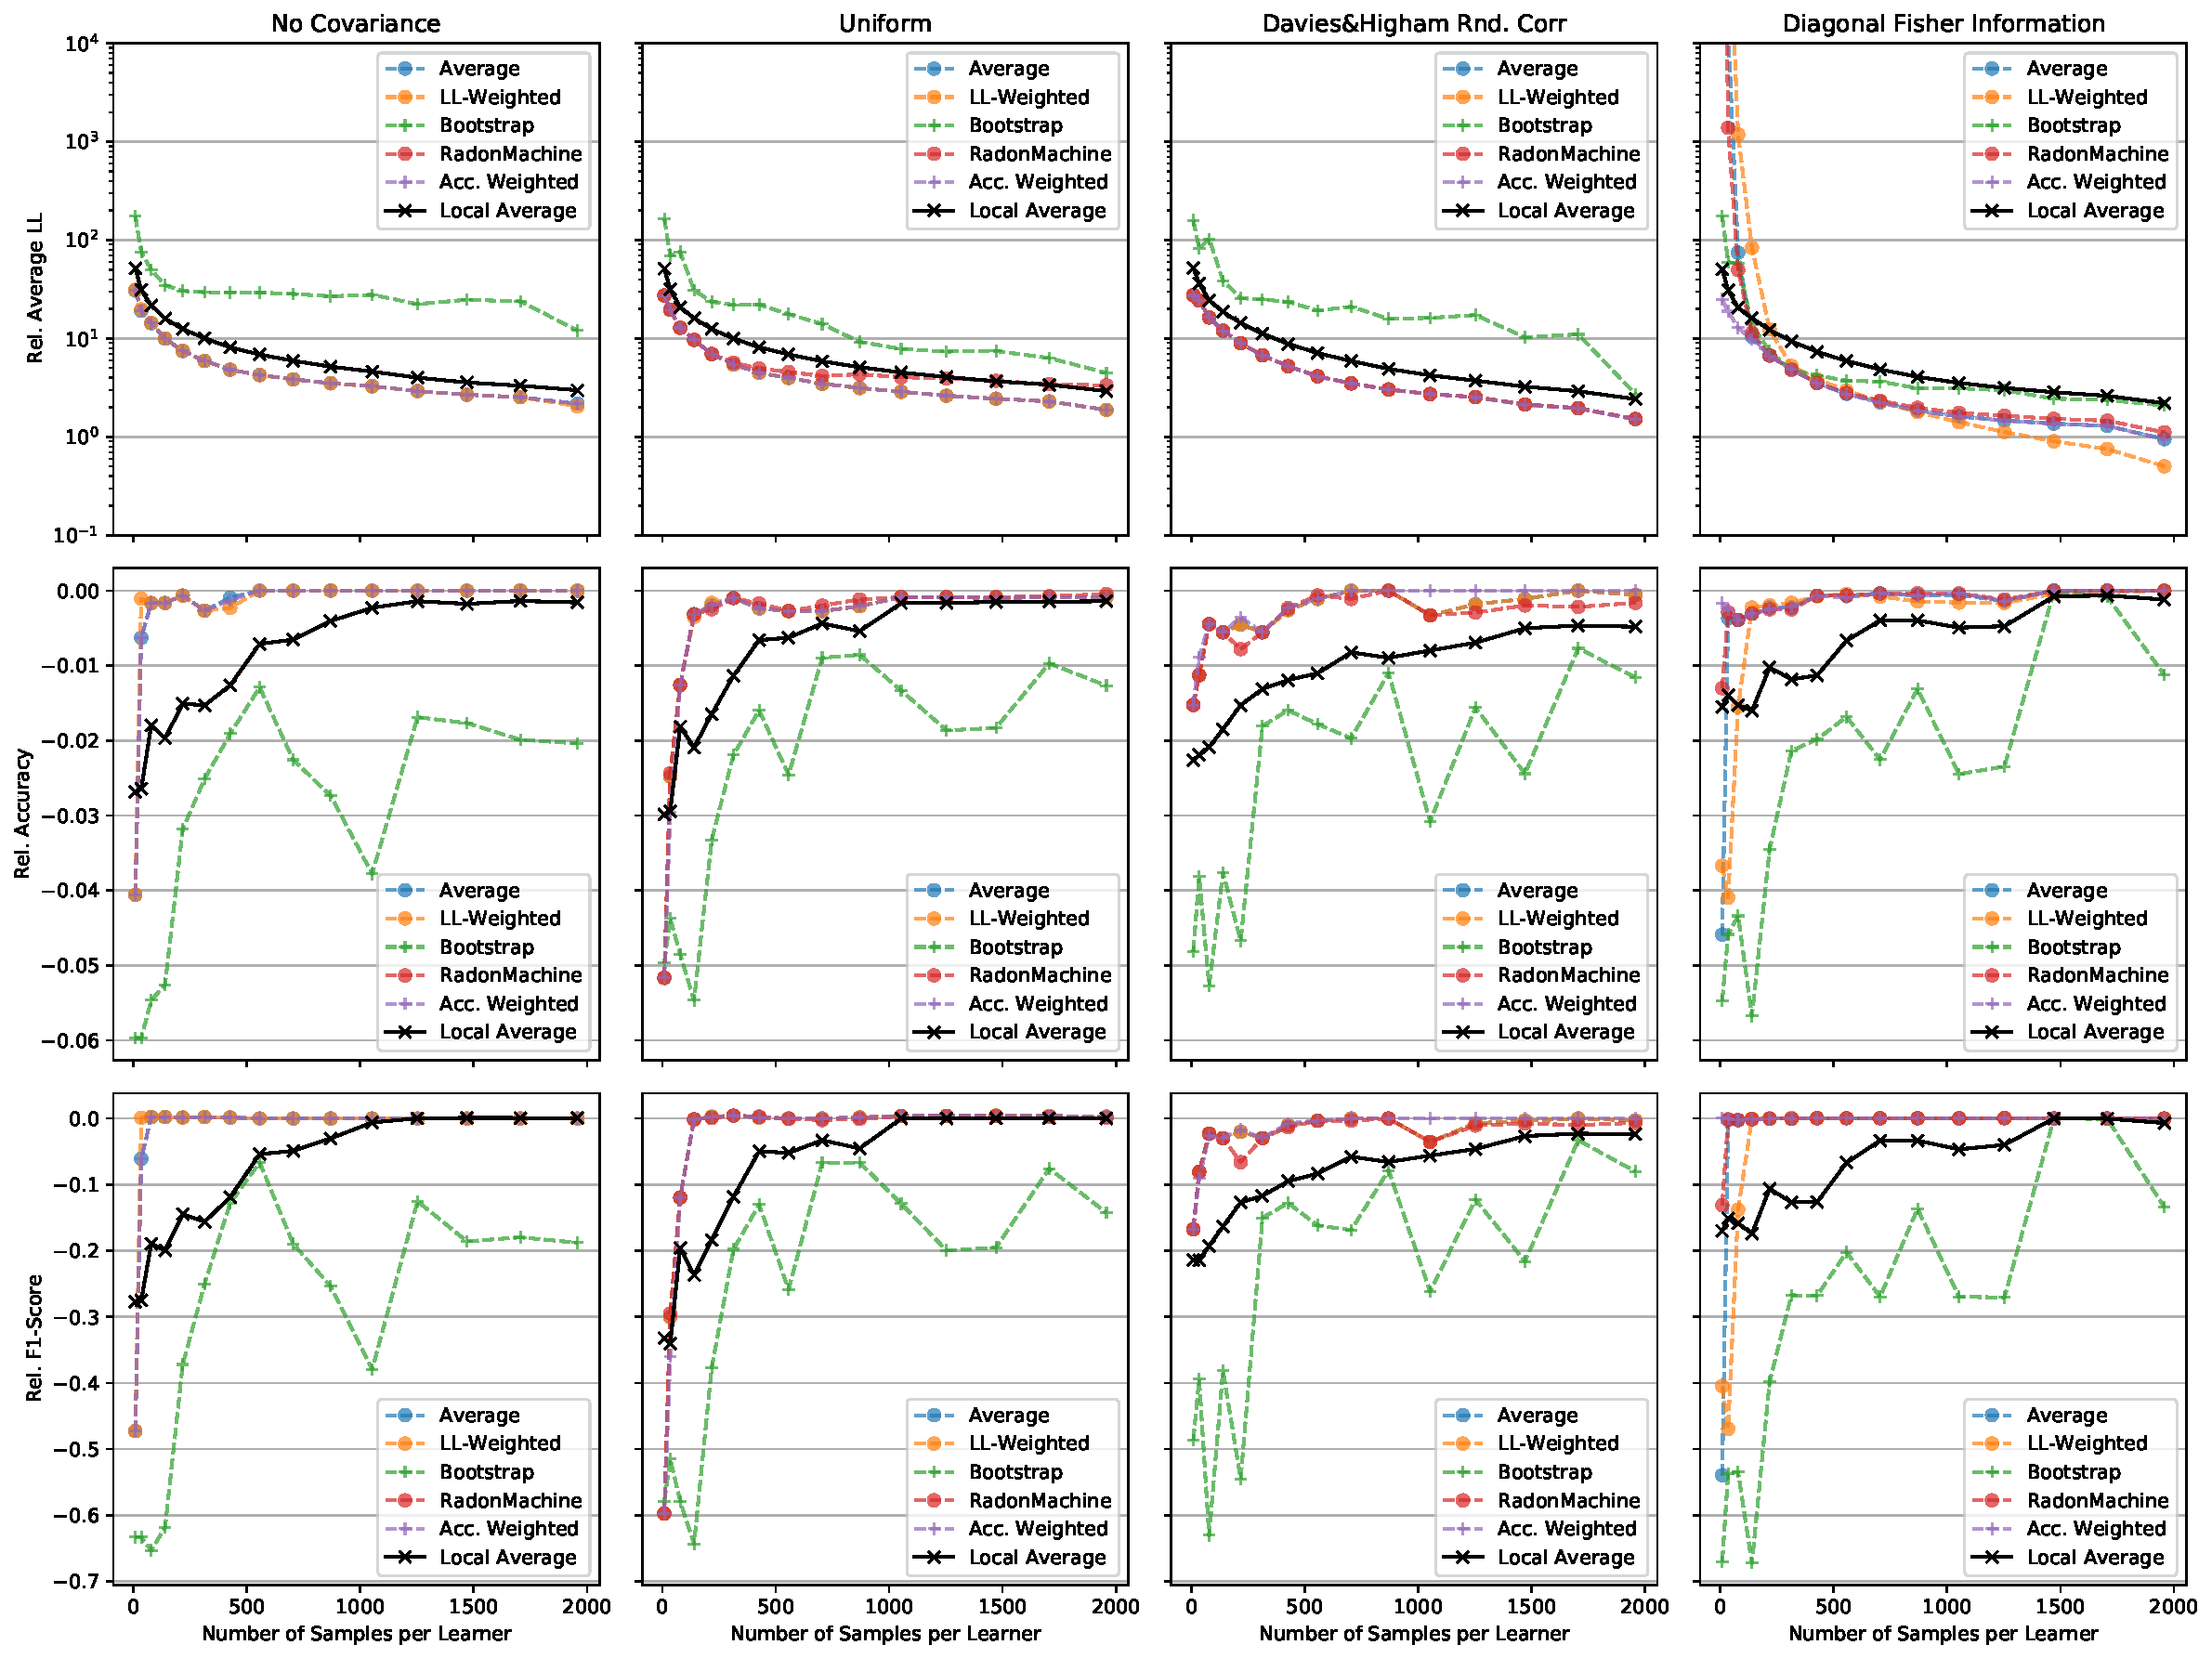
\includegraphics[height=\dimexpr \textheight - 4\baselineskip\relax]{kapitel/figures/dota2_l2_0.1_neg_relative.pdf}
            \caption[Dota2 plots with l2 regularization and $\epsilon=0.1$]{Experimental results on the Dota2 data set for $k=10$ distributed learners. Each plot represents a combination of metric and covariance matrix used for sampling. Values on the x-Axis are the number of samples available on each learner. The top row shows the relative negative average log likelihood $\ell(\tilde{\vect{\theta}}; \mathcal{D}) - \ell(\hat{\vect{\theta}}; \mathcal{D})$ for each aggregate. Second and third row show accuracy and F1-score relative to the baseline on the test set.}
            \label{fig:analysis12}
        \end{figure}
    \end{landscape}

\section{Independence Structures}
\label{sec:apdx:struc}

\begin{figure}[!htb]
\center
\centering
\textbf{Independence Graph for Susy generated by the Chow-Liu algorithm}\par\medskip
\begin{tikzpicture}
\clip (0,0) rectangle (17.0,15.0);
\Vertex[x=5.611,y=13.063,size=0.5,color=blue,opacity=0.7]{0}
\Vertex[x=7.389,y=12.774,size=0.5,color=tuorange,opacity=0.7]{2}
\Vertex[x=9.526,y=11.806,size=0.5,color=tugreen,opacity=0.7]{1}
\Vertex[x=11.448,y=10.109,size=0.5,color=tuorange,opacity=0.7]{11}
\Vertex[x=6.818,y=14.000,size=0.5,color=tugreen,opacity=0.7]{5}
\Vertex[x=13.820,y=3.181,size=0.5,color=tugreen,opacity=0.7]{3}
\Vertex[x=12.432,y=1.605,size=0.5,color=tuorange,opacity=0.7]{6}
\Vertex[x=13.892,y=5.464,size=0.5,color=tuorange,opacity=0.7]{8}
\Vertex[x=12.896,y=7.850,size=0.5,color=tugreen,opacity=0.7]{4}
\Vertex[x=9.531,y=5.061,size=0.5,color=tugreen,opacity=0.7]{7}
\Vertex[x=6.976,y=4.562,size=0.5,color=tuorange,opacity=0.7]{9}
\Vertex[x=11.070,y=4.835,size=0.5,color=tuorange,opacity=0.7]{10}
\Vertex[x=10.298,y=7.228,size=0.5,color=tuorange,opacity=0.7]{12}
\Vertex[x=8.875,y=2.780,size=0.5,color=tuorange,opacity=0.7]{13}
\Vertex[x=11.669,y=6.020,size=0.5,color=tuorange,opacity=0.7]{17}
\Vertex[x=4.788,y=3.995,size=0.5,color=tugreen,opacity=0.7]{16}
\Vertex[x=11.329,y=8.920,size=0.5,color=tugreen,opacity=0.7]{15}
\Vertex[x=8.393,y=1.000,size=0.5,color=tugreen,opacity=0.7]{18}
\Vertex[x=3.108,y=3.487,size=0.5,color=tuorange,opacity=0.7]{14}
\Edge[,lw=0.1,color=black](0)(2)
\Edge[,lw=0.1,color=black](2)(1)
\Edge[,lw=0.1,color=black](2)(5)
\Edge[,lw=0.1,color=black](1)(11)
\Edge[,lw=0.1,color=black](11)(4)
\Edge[,lw=0.1,color=black](11)(15)
\Edge[,lw=0.1,color=black](3)(6)
\Edge[,lw=0.1,color=black](3)(8)
\Edge[,lw=0.1,color=black](8)(4)
\Edge[,lw=0.1,color=black](7)(9)
\Edge[,lw=0.1,color=black](7)(10)
\Edge[,lw=0.1,color=black](7)(12)
\Edge[,lw=0.1,color=black](7)(13)
\Edge[,lw=0.1,color=black](7)(17)
\Edge[,lw=0.1,color=black](9)(16)
\Edge[,lw=0.1,color=black](12)(15)
\Edge[,lw=0.1,color=black](13)(18)
\Edge[,lw=0.1,color=black](16)(14)
\end{tikzpicture}
\caption[Approximated independence structure of the Susy data set]{Tree estimated with the Chow-Liu algorithm. Neighboring nodes are displayed with alternating colors generated from a 2-Coloring algorithm to improve visibility. The root, which is the random variable for the labels, is shown in blue.}
\label{fig:susy_ind}
\end{figure}
\begin{figure}[!htb]
    \center
    \textbf{Independence Graph for Covertype generated by the Chow-Liu algorithm}\par\medskip
    \resizebox{\linewidth}{!}{%
    \begin{tikzpicture}
        \clip (0,0) rectangle (17.0,15.0);
        \Vertex[x=12.637,y=6.951,size=0.5,color=tuorange,opacity=0.7]{0}
        \Vertex[x=13.224,y=8.670,size=0.5,color=tugreen,opacity=0.7]{3}
        \Vertex[x=14.502,y=6.725,size=0.5,color=tugreen,opacity=0.7]{5}
        \Vertex[x=12.634,y=8.090,size=0.5,color=tugreen,opacity=0.7]{9}
        \Vertex[x=10.487,y=5.452,size=0.5,color=blue,opacity=0.7]{54}
        \Vertex[x=8.715,y=11.565,size=0.5,color=tugreen,opacity=0.7]{1}
        \Vertex[x=7.132,y=12.694,size=0.5,color=tuorange,opacity=0.7]{6}
        \Vertex[x=10.448,y=11.497,size=0.5,color=tuorange,opacity=0.7]{7}
        \Vertex[x=8.610,y=10.130,size=0.5,color=tuorange,opacity=0.7]{8}
        \Vertex[x=12.001,y=11.238,size=0.5,color=tugreen,opacity=0.7]{2}
        \Vertex[x=13.029,y=10.213,size=0.5,color=tuorange,opacity=0.7]{4}
        \Vertex[x=15.279,y=6.087,size=0.5,color=tuorange,opacity=0.7]{14}
        \Vertex[x=15.747,y=6.864,size=0.5,color=tuorange,opacity=0.7]{15}
        \Vertex[x=5.924,y=13.037,size=0.5,color=tugreen,opacity=0.7]{10}
        \Vertex[x=7.538,y=13.901,size=0.5,color=tugreen,opacity=0.7]{11}
        \Vertex[x=6.827,y=14.000,size=0.5,color=tugreen,opacity=0.7]{12}
        \Vertex[x=5.999,y=11.852,size=0.5,color=tugreen,opacity=0.7]{13}
        \Vertex[x=6.440,y=12.705,size=0.5,color=tugreen,opacity=0.7]{16}
        \Vertex[x=5.108,y=11.775,size=0.5,color=tuorange,opacity=0.7]{43}
        \Vertex[x=10.085,y=7.026,size=0.5,color=tuorange,opacity=0.7]{17}
        \Vertex[x=2.368,y=11.619,size=0.5,color=tuorange,opacity=0.7]{18}
        \Vertex[x=1.253,y=12.024,size=0.5,color=tugreen,opacity=0.7]{19}
        \Vertex[x=1.757,y=12.689,size=0.5,color=tugreen,opacity=0.7]{20}
        \Vertex[x=3.959,y=10.329,size=0.5,color=tugreen,opacity=0.7]{27}
        \Vertex[x=10.642,y=6.917,size=0.5,color=tuorange,opacity=0.7]{21}
        \Vertex[x=5.790,y=4.399,size=0.5,color=tuorange,opacity=0.7]{22}
        \Vertex[x=6.961,y=3.509,size=0.5,color=tugreen,opacity=0.7]{32}
        \Vertex[x=8.659,y=2.745,size=0.5,color=tuorange,opacity=0.7]{23}
        \Vertex[x=6.917,y=5.374,size=0.5,color=tugreen,opacity=0.7]{33}
        \Vertex[x=8.551,y=1.000,size=0.5,color=tugreen,opacity=0.7]{34}
        \Vertex[x=9.886,y=3.161,size=0.5,color=tugreen,opacity=0.7]{35}
        \Vertex[x=7.809,y=2.199,size=0.5,color=tugreen,opacity=0.7]{36}
        \Vertex[x=7.463,y=2.745,size=0.5,color=tugreen,opacity=0.7]{37}
        \Vertex[x=9.674,y=1.333,size=0.5,color=tugreen,opacity=0.7]{38}
        \Vertex[x=10.054,y=1.846,size=0.5,color=tugreen,opacity=0.7]{39}
        \Vertex[x=9.150,y=1.055,size=0.5,color=tugreen,opacity=0.7]{40}
        \Vertex[x=9.626,y=2.552,size=0.5,color=tugreen,opacity=0.7]{41}
        \Vertex[x=7.220,y=2.063,size=0.5,color=tugreen,opacity=0.7]{45}
        \Vertex[x=7.524,y=1.524,size=0.5,color=tugreen,opacity=0.7]{46}
        \Vertex[x=10.202,y=2.467,size=0.5,color=tugreen,opacity=0.7]{47}
        \Vertex[x=9.216,y=3.550,size=0.5,color=tugreen,opacity=0.7]{48}
        \Vertex[x=7.974,y=1.135,size=0.5,color=tugreen,opacity=0.7]{49}
        \Vertex[x=9.432,y=1.871,size=0.5,color=tugreen,opacity=0.7]{50}
        \Vertex[x=8.865,y=1.565,size=0.5,color=tugreen,opacity=0.7]{51}
        \Vertex[x=8.226,y=1.652,size=0.5,color=tugreen,opacity=0.7]{52}
        \Vertex[x=8.174,y=3.472,size=0.5,color=tugreen,opacity=0.7]{53}
        \Vertex[x=5.308,y=8.004,size=0.5,color=tuorange,opacity=0.7]{24}
        \Vertex[x=6.057,y=8.782,size=0.5,color=tugreen,opacity=0.7]{25}
        \Vertex[x=6.176,y=7.988,size=0.5,color=tugreen,opacity=0.7]{26}
        \Vertex[x=4.566,y=8.365,size=0.5,color=tugreen,opacity=0.7]{28}
        \Vertex[x=4.210,y=7.479,size=0.5,color=tugreen,opacity=0.7]{29}
        \Vertex[x=4.782,y=8.969,size=0.5,color=tugreen,opacity=0.7]{30}
        \Vertex[x=5.359,y=8.909,size=0.5,color=tugreen,opacity=0.7]{31}
        \Vertex[x=3.691,y=9.682,size=0.5,color=tuorange,opacity=0.7]{42}
        \Vertex[x=2.783,y=10.701,size=0.5,color=tuorange,opacity=0.7]{44}
        \Edge[](0)(3)
        \Edge[](0)(5)
        \Edge[](0)(9)
        \Edge[](0)(54)
        \Edge[](3)(4)
        \Edge[](5)(14)
        \Edge[](5)(15)
        \Edge[](54)(17)
        \Edge[](54)(21)
        \Edge[](54)(23)
        \Edge[](1)(6)
        \Edge[](1)(7)
        \Edge[](1)(8)
        \Edge[](6)(10)
        \Edge[](6)(11)
        \Edge[](6)(12)
        \Edge[](6)(13)
        \Edge[](7)(2)
        \Edge[](2)(4)
        \Edge[](16)(43)
        \Edge[](43)(27)
        \Edge[](18)(19)
        \Edge[](18)(20)
        \Edge[](18)(27)
        \Edge[](27)(24)
        \Edge[](27)(42)
        \Edge[](27)(44)
        \Edge[](22)(32)
        \Edge[](32)(23)
        \Edge[](23)(33)
        \Edge[](23)(34)
        \Edge[](23)(35)
        \Edge[](23)(36)
        \Edge[](23)(37)
        \Edge[](23)(38)
        \Edge[](23)(39)
        \Edge[](23)(40)
        \Edge[](23)(41)
        \Edge[](23)(45)
        \Edge[](23)(46)
        \Edge[](23)(47)
        \Edge[](23)(48)
        \Edge[](23)(49)
        \Edge[](23)(50)
        \Edge[](23)(51)
        \Edge[](23)(52)
        \Edge[](23)(53)
        \Edge[](33)(24)
        \Edge[](24)(25)
        \Edge[](24)(26)
        \Edge[](24)(28)
        \Edge[](24)(29)
        \Edge[](24)(30)
        \Edge[](24)(31)
        \end{tikzpicture}%
    }
        \caption[Approximated independence structure of the Covertype data set]{tree estimated with the Chow-Liu algorithm. Neighboring nodes are displayed with alternating colors generated from a 2-Coloring algorithm to improve visibility. The root, which is the random variable for the labels, is shown in blue.}
        \label{fig:covertype_ind}
\end{figure}
\begin{figure}[!htb]
    \center
    \centering
    \textbf{Independence Graph for Dota2 generated by the Chow-Liu algorithm}\par\medskip
    \begin{tikzpicture}
        \clip (0,0) rectangle (17.0,15.0);
        \Vertex[x=11.316,y=3.353,size=0.5,color=red,opacity=0.7]{0}
        \Vertex[x=11.193,y=2.043,size=0.5,color=tuorange,opacity=0.7]{27}
        \Vertex[x=11.456,y=5.259,size=0.5,color=tuorange,opacity=0.7]{36}
        \Vertex[x=11.696,y=7.743,size=0.5,color=tugreen,opacity=0.7]{1}
        \Vertex[x=6.131,y=8.696,size=0.5,color=tuorange,opacity=0.7]{2}
        \Vertex[x=11.361,y=6.194,size=0.5,color=tuorange,opacity=0.7]{6}
        \Vertex[x=13.171,y=8.568,size=0.5,color=tuorange,opacity=0.7]{7}
        \Vertex[x=12.637,y=8.555,size=0.5,color=tuorange,opacity=0.7]{8}
        \Vertex[x=8.865,y=5.803,size=0.5,color=tuorange,opacity=0.7]{9}
        \Vertex[x=13.491,y=9.260,size=0.5,color=tuorange,opacity=0.7]{10}
        \Vertex[x=12.661,y=7.890,size=0.5,color=tuorange,opacity=0.7]{13}
        \Vertex[x=12.666,y=9.164,size=0.5,color=tuorange,opacity=0.7]{14}
        \Vertex[x=12.491,y=6.838,size=0.5,color=tuorange,opacity=0.7]{16}
        \Vertex[x=10.282,y=7.825,size=0.5,color=tuorange,opacity=0.7]{19}
        \Vertex[x=11.971,y=8.736,size=0.5,color=tuorange,opacity=0.7]{20}
        \Vertex[x=13.948,y=7.083,size=0.5,color=tuorange,opacity=0.7]{21}
        \Vertex[x=13.323,y=8.130,size=0.5,color=tuorange,opacity=0.7]{23}
        \Vertex[x=10.855,y=9.717,size=0.5,color=tuorange,opacity=0.7]{28}
        \Vertex[x=11.864,y=9.281,size=0.5,color=tuorange,opacity=0.7]{30}
        \Vertex[x=11.305,y=7.095,size=0.5,color=tuorange,opacity=0.7]{31}
        \Vertex[x=11.559,y=8.948,size=0.5,color=tuorange,opacity=0.7]{32}
        \Vertex[x=12.681,y=6.503,size=0.5,color=tuorange,opacity=0.7]{33}
        \Vertex[x=13.011,y=6.806,size=0.5,color=tuorange,opacity=0.7]{34}
        \Vertex[x=12.061,y=5.558,size=0.5,color=tuorange,opacity=0.7]{37}
        \Vertex[x=10.077,y=8.779,size=0.5,color=tuorange,opacity=0.7]{38}
        \Vertex[x=11.436,y=8.463,size=0.5,color=tuorange,opacity=0.7]{39}
        \Vertex[x=10.898,y=8.122,size=0.5,color=tuorange,opacity=0.7]{40}
        \Vertex[x=12.915,y=8.864,size=0.5,color=tuorange,opacity=0.7]{42}
        \Vertex[x=11.013,y=6.699,size=0.5,color=tuorange,opacity=0.7]{43}
        \Vertex[x=13.913,y=8.553,size=0.5,color=tuorange,opacity=0.7]{47}
        \Vertex[x=12.256,y=9.304,size=0.5,color=tuorange,opacity=0.7]{49}
        \Vertex[x=12.957,y=8.229,size=0.5,color=tuorange,opacity=0.7]{54}
        \Vertex[x=11.009,y=8.673,size=0.5,color=tuorange,opacity=0.7]{56}
        \Vertex[x=11.503,y=6.591,size=0.5,color=tuorange,opacity=0.7]{59}
        \Vertex[x=13.007,y=7.627,size=0.5,color=tuorange,opacity=0.7]{60}
        \Vertex[x=10.296,y=7.400,size=0.5,color=tuorange,opacity=0.7]{61}
        \Vertex[x=11.933,y=9.976,size=0.5,color=tuorange,opacity=0.7]{62}
        \Vertex[x=13.364,y=7.729,size=0.5,color=tuorange,opacity=0.7]{68}
        \Vertex[x=12.602,y=10.432,size=0.5,color=tuorange,opacity=0.7]{71}
        \Vertex[x=10.615,y=6.612,size=0.5,color=tuorange,opacity=0.7]{72}
        \Vertex[x=14.056,y=7.811,size=0.5,color=tuorange,opacity=0.7]{73}
        \Vertex[x=13.256,y=6.044,size=0.5,color=tuorange,opacity=0.7]{78}
        \Vertex[x=10.779,y=7.168,size=0.5,color=tuorange,opacity=0.7]{81}
        \Vertex[x=11.998,y=6.537,size=0.5,color=tuorange,opacity=0.7]{82}
        \Vertex[x=12.301,y=6.300,size=0.5,color=tuorange,opacity=0.7]{83}
        \Vertex[x=13.279,y=7.270,size=0.5,color=tuorange,opacity=0.7]{85}
        \Vertex[x=12.354,y=8.917,size=0.5,color=tuorange,opacity=0.7]{86}
        \Vertex[x=10.437,y=8.216,size=0.5,color=tuorange,opacity=0.7]{88}
        \Vertex[x=11.981,y=6.991,size=0.5,color=tuorange,opacity=0.7]{90}
        \Vertex[x=13.671,y=6.509,size=0.5,color=tuorange,opacity=0.7]{91}
        \Vertex[x=10.400,y=6.980,size=0.5,color=tuorange,opacity=0.7]{95}
        \Vertex[x=12.461,y=7.366,size=0.5,color=tuorange,opacity=0.7]{98}
        \Vertex[x=11.013,y=9.072,size=0.5,color=tuorange,opacity=0.7]{99}
        \Vertex[x=10.626,y=8.672,size=0.5,color=tuorange,opacity=0.7]{101}
        \Vertex[x=11.792,y=6.184,size=0.5,color=tuorange,opacity=0.7]{104}
        \Vertex[x=10.968,y=6.304,size=0.5,color=tuorange,opacity=0.7]{105}
        \Vertex[x=12.724,y=5.713,size=0.5,color=tuorange,opacity=0.7]{106}
        \Vertex[x=11.418,y=9.298,size=0.5,color=tuorange,opacity=0.7]{113}
        \Vertex[x=10.745,y=7.646,size=0.5,color=tuorange,opacity=0.7]{114}
        \Vertex[x=12.894,y=7.165,size=0.5,color=tuorange,opacity=0.7]{115}
        \Vertex[x=12.253,y=8.248,size=0.5,color=tuorange,opacity=0.7]{116}
        \Vertex[x=3.205,y=8.134,size=0.5,color=tugreen,opacity=0.7]{3}
        \Vertex[x=4.246,y=9.072,size=0.5,color=tugreen,opacity=0.7]{5}
        \Vertex[x=5.692,y=8.175,size=0.5,color=tugreen,opacity=0.7]{17}
        \Vertex[x=5.187,y=7.893,size=0.5,color=tugreen,opacity=0.7]{18}
        \Vertex[x=5.604,y=7.629,size=0.5,color=tugreen,opacity=0.7]{22}
        \Vertex[x=6.193,y=9.801,size=0.5,color=tugreen,opacity=0.7]{50}
        \Vertex[x=5.207,y=8.358,size=0.5,color=tugreen,opacity=0.7]{52}
        \Vertex[x=6.104,y=7.815,size=0.5,color=tugreen,opacity=0.7]{63}
        \Vertex[x=4.809,y=8.370,size=0.5,color=tugreen,opacity=0.7]{64}
        \Vertex[x=5.516,y=9.557,size=0.5,color=tugreen,opacity=0.7]{75}
        \Vertex[x=4.460,y=11.054,size=0.5,color=tugreen,opacity=0.7]{77}
        \Vertex[x=4.872,y=8.834,size=0.5,color=tugreen,opacity=0.7]{80}
        \Vertex[x=5.080,y=9.277,size=0.5,color=tugreen,opacity=0.7]{84}
        \Vertex[x=5.926,y=9.378,size=0.5,color=tugreen,opacity=0.7]{92}
        \Vertex[x=4.642,y=7.499,size=0.5,color=tugreen,opacity=0.7]{103}
        \Vertex[x=4.812,y=9.977,size=0.5,color=tugreen,opacity=0.7]{107}
        \Vertex[x=5.372,y=8.901,size=0.5,color=tugreen,opacity=0.7]{112}
        \Vertex[x=1.886,y=7.757,size=0.5,color=tuorange,opacity=0.7]{12}
        \Vertex[x=1.750,y=8.095,size=0.5,color=tuorange,opacity=0.7]{55}
        \Vertex[x=1.923,y=8.400,size=0.5,color=tuorange,opacity=0.7]{93}
        \Vertex[x=2.089,y=7.445,size=0.5,color=tuorange,opacity=0.7]{108}
        \Vertex[x=4.321,y=3.743,size=0.5,color=tuorange,opacity=0.7]{4}
        \Vertex[x=2.595,y=3.948,size=0.5,color=tugreen,opacity=0.7]{57}
        \Vertex[x=6.336,y=4.012,size=0.5,color=tugreen,opacity=0.7]{96}
        \Vertex[x=2.949,y=9.392,size=0.5,color=tuorange,opacity=0.7]{100}
        \Vertex[x=7.895,y=5.875,size=0.5,color=tugreen,opacity=0.7]{70}
        \Vertex[x=14.708,y=10.231,size=0.5,color=tugreen,opacity=0.7]{87}
        \Vertex[x=5.360,y=2.182,size=0.5,color=tuorange,opacity=0.7]{11}
        \Vertex[x=4.579,y=1.226,size=0.5,color=tugreen,opacity=0.7]{15}
        \Vertex[x=5.008,y=1.000,size=0.5,color=tugreen,opacity=0.7]{58}
        \Vertex[x=15.446,y=6.594,size=0.5,color=tugreen,opacity=0.7]{109}
        \Vertex[x=10.206,y=11.004,size=0.5,color=tugreen,opacity=0.7]{24}
        \Vertex[x=3.771,y=12.270,size=0.5,color=tuorange,opacity=0.7]{25}
        \Vertex[x=12.301,y=4.094,size=0.5,color=tugreen,opacity=0.7]{26}
        \Vertex[x=13.256,y=12.661,size=0.5,color=tugreen,opacity=0.7]{29}
        \Vertex[x=13.851,y=13.858,size=0.5,color=tuorange,opacity=0.7]{48}
        \Vertex[x=13.383,y=14.000,size=0.5,color=tuorange,opacity=0.7]{67}
        \Vertex[x=3.041,y=12.214,size=0.5,color=tugreen,opacity=0.7]{35}
        \Vertex[x=3.997,y=11.015,size=0.5,color=tuorange,opacity=0.7]{44}
        \Vertex[x=2.077,y=13.113,size=0.5,color=tuorange,opacity=0.7]{65}
        \Vertex[x=9.012,y=9.408,size=0.5,color=tugreen,opacity=0.7]{41}
        \Vertex[x=5.126,y=10.179,size=0.5,color=tugreen,opacity=0.7]{45}
        \Vertex[x=4.493,y=12.237,size=0.5,color=tuorange,opacity=0.7]{46}
        \Vertex[x=15.397,y=9.068,size=0.5,color=tugreen,opacity=0.7]{51}
        \Vertex[x=12.072,y=11.478,size=0.5,color=tugreen,opacity=0.7]{53}
        \Vertex[x=1.362,y=4.667,size=0.5,color=tuorange,opacity=0.7]{74}
        \Vertex[x=3.475,y=11.884,size=0.5,color=tuorange,opacity=0.7]{66}
        \Vertex[x=5.965,y=3.371,size=0.5,color=tuorange,opacity=0.7]{69}
        \Vertex[x=15.638,y=7.842,size=0.5,color=tugreen,opacity=0.7]{110}
        \Vertex[x=4.133,y=12.007,size=0.5,color=tuorange,opacity=0.7]{76}
        \Vertex[x=3.197,y=11.510,size=0.5,color=tuorange,opacity=0.7]{79}
        \Vertex[x=14.283,y=4.880,size=0.5,color=tugreen,opacity=0.7]{89}
        \Vertex[x=14.977,y=5.643,size=0.5,color=tugreen,opacity=0.7]{94}
        \Vertex[x=5.372,y=4.142,size=0.5,color=tuorange,opacity=0.7]{97}
        \Vertex[x=13.406,y=4.341,size=0.5,color=tugreen,opacity=0.7]{102}
        \Vertex[x=3.624,y=6.631,size=0.5,color=tuorange,opacity=0.7]{111}
        \Edge[,lw=0.1,color=black](0)(27)
        \Edge[,lw=0.1,color=black](0)(36)
        \Edge[,lw=0.1,color=black](36)(1)
        \Edge[,lw=0.1,color=black](1)(2)
        \Edge[,lw=0.1,color=black](1)(6)
        \Edge[,lw=0.1,color=black](1)(7)
        \Edge[,lw=0.1,color=black](1)(8)
        \Edge[,lw=0.1,color=black](1)(9)
        \Edge[,lw=0.1,color=black](1)(10)
        \Edge[,lw=0.1,color=black](1)(13)
        \Edge[,lw=0.1,color=black](1)(14)
        \Edge[,lw=0.1,color=black](1)(16)
        \Edge[,lw=0.1,color=black](1)(19)
        \Edge[,lw=0.1,color=black](1)(20)
        \Edge[,lw=0.1,color=black](1)(21)
        \Edge[,lw=0.1,color=black](1)(23)
        \Edge[,lw=0.1,color=black](1)(28)
        \Edge[,lw=0.1,color=black](1)(30)
        \Edge[,lw=0.1,color=black](1)(31)
        \Edge[,lw=0.1,color=black](1)(32)
        \Edge[,lw=0.1,color=black](1)(33)
        \Edge[,lw=0.1,color=black](1)(34)
        \Edge[,lw=0.1,color=black](1)(37)
        \Edge[,lw=0.1,color=black](1)(38)
        \Edge[,lw=0.1,color=black](1)(39)
        \Edge[,lw=0.1,color=black](1)(40)
        \Edge[,lw=0.1,color=black](1)(42)
        \Edge[,lw=0.1,color=black](1)(43)
        \Edge[,lw=0.1,color=black](1)(47)
        \Edge[,lw=0.1,color=black](1)(49)
        \Edge[,lw=0.1,color=black](1)(54)
        \Edge[,lw=0.1,color=black](1)(56)
        \Edge[,lw=0.1,color=black](1)(59)
        \Edge[,lw=0.1,color=black](1)(60)
        \Edge[,lw=0.1,color=black](1)(61)
        \Edge[,lw=0.1,color=black](1)(62)
        \Edge[,lw=0.1,color=black](1)(68)
        \Edge[,lw=0.1,color=black](1)(71)
        \Edge[,lw=0.1,color=black](1)(72)
        \Edge[,lw=0.1,color=black](1)(73)
        \Edge[,lw=0.1,color=black](1)(78)
        \Edge[,lw=0.1,color=black](1)(81)
        \Edge[,lw=0.1,color=black](1)(82)
        \Edge[,lw=0.1,color=black](1)(83)
        \Edge[,lw=0.1,color=black](1)(85)
        \Edge[,lw=0.1,color=black](1)(86)
        \Edge[,lw=0.1,color=black](1)(88)
        \Edge[,lw=0.1,color=black](1)(90)
        \Edge[,lw=0.1,color=black](1)(91)
        \Edge[,lw=0.1,color=black](1)(95)
        \Edge[,lw=0.1,color=black](1)(98)
        \Edge[,lw=0.1,color=black](1)(99)
        \Edge[,lw=0.1,color=black](1)(101)
        \Edge[,lw=0.1,color=black](1)(104)
        \Edge[,lw=0.1,color=black](1)(105)
        \Edge[,lw=0.1,color=black](1)(106)
        \Edge[,lw=0.1,color=black](1)(113)
        \Edge[,lw=0.1,color=black](1)(114)
        \Edge[,lw=0.1,color=black](1)(115)
        \Edge[,lw=0.1,color=black](1)(116)
        \Edge[,lw=0.1,color=black](2)(3)
        \Edge[,lw=0.1,color=black](2)(5)
        \Edge[,lw=0.1,color=black](2)(17)
        \Edge[,lw=0.1,color=black](2)(18)
        \Edge[,lw=0.1,color=black](2)(22)
        \Edge[,lw=0.1,color=black](2)(50)
        \Edge[,lw=0.1,color=black](2)(52)
        \Edge[,lw=0.1,color=black](2)(63)
        \Edge[,lw=0.1,color=black](2)(64)
        \Edge[,lw=0.1,color=black](2)(75)
        \Edge[,lw=0.1,color=black](2)(77)
        \Edge[,lw=0.1,color=black](2)(80)
        \Edge[,lw=0.1,color=black](2)(84)
        \Edge[,lw=0.1,color=black](2)(92)
        \Edge[,lw=0.1,color=black](2)(103)
        \Edge[,lw=0.1,color=black](2)(107)
        \Edge[,lw=0.1,color=black](2)(112)
        \Edge[,lw=0.1,color=black](9)(70)
        \Edge[,lw=0.1,color=black](9)(96)
        \Edge[,lw=0.1,color=black](10)(87)
        \Edge[,lw=0.1,color=black](21)(109)
        \Edge[,lw=0.1,color=black](28)(24)
        \Edge[,lw=0.1,color=black](37)(26)
        \Edge[,lw=0.1,color=black](38)(41)
        \Edge[,lw=0.1,color=black](47)(51)
        \Edge[,lw=0.1,color=black](62)(53)
        \Edge[,lw=0.1,color=black](71)(29)
        \Edge[,lw=0.1,color=black](73)(110)
        \Edge[,lw=0.1,color=black](78)(89)
        \Edge[,lw=0.1,color=black](91)(94)
        \Edge[,lw=0.1,color=black](106)(102)
        \Edge[,lw=0.1,color=black](3)(12)
        \Edge[,lw=0.1,color=black](3)(55)
        \Edge[,lw=0.1,color=black](3)(93)
        \Edge[,lw=0.1,color=black](3)(108)
        \Edge[,lw=0.1,color=black](5)(100)
        \Edge[,lw=0.1,color=black](77)(25)
        \Edge[,lw=0.1,color=black](77)(46)
        \Edge[,lw=0.1,color=black](77)(66)
        \Edge[,lw=0.1,color=black](77)(76)
        \Edge[,lw=0.1,color=black](77)(79)
        \Edge[,lw=0.1,color=black](103)(111)
        \Edge[,lw=0.1,color=black](107)(44)
        \Edge[,lw=0.1,color=black](4)(57)
        \Edge[,lw=0.1,color=black](4)(96)
        \Edge[,lw=0.1,color=black](57)(74)
        \Edge[,lw=0.1,color=black](96)(11)
        \Edge[,lw=0.1,color=black](96)(69)
        \Edge[,lw=0.1,color=black](96)(97)
        \Edge[,lw=0.1,color=black](11)(15)
        \Edge[,lw=0.1,color=black](11)(58)
        \Edge[,lw=0.1,color=black](29)(48)
        \Edge[,lw=0.1,color=black](29)(67)
        \Edge[,lw=0.1,color=black](35)(44)
        \Edge[,lw=0.1,color=black](35)(65)
        \Edge[,lw=0.1,color=black](44)(45)
        \end{tikzpicture}
    \caption[Approximated independence structure of the Dota2 data set]{Tree estimated with the Chow-Liu algorithm. Neighboring nodes are displayed with alternating colors generated from a 2-Coloring algorithm to improve visibility. The root, which is the random variable for the labels, is shown in blue.}
    \label{fig:dota_ind}
    \end{figure}

\clearpage
\section{Parameter Variance Tables}
The standard deviations in tables \ref{tab:avg_std_01},~\ref{tab:std_std_005},~\ref{tab:std_std_01},~\ref{tab_avg_std_005} are computed \wrt to each dimension and each set of local parameter vectors.
We compute the mean of all variances for all experiments with the same regularization type and over all local model parameters with the same number of samples:
\begin{equation}
    \label{eq:meanvar}
    \hat{\sigma}_{p,r} = \sqrt{\frac{1}{p} \sum_{i=1}^p \text{mean}(\text{var}((\vect{\Theta}^{i_r}))},
\end{equation}
where $p=4$ is the number of, $r$ is the number of samples, and $\Theta$ is the set of local parameter vectors.
We obtain the variance of the variances analogous by replacing the inner average with the variance:
\begin{equation}
    \label{eq:varvar}
    \hat{\sigma}_{p,r} = \sqrt{\frac{1}{p} \sum_{i=1}^p \text{var}(\text{var}((\vect{\Theta}^{i_r}))},
\end{equation}
where the inner variance is always taken \wrt to each dimension and the outer mean and variance are compted over all elements.

\begin{table}[!htb]
    \centering
    \caption[Average local parameter std. for $\epsilon=0.1$]{This table shows the total average standard deviation (\eq~\ref{eq:meanvar}) for $\epsilon=0.1$ across local model parameters $\vect{\theta}^i$ from all splits, in ascending order \wrt the sample size. We observe that the std. steadily decreases, but does not achieve the same score as the global model. The std. is computed \wrt all models with the same number of samples and for each parameter dimension individually.
    }
    \label{tab:avg_std_01}
    \resizebox{\linewidth}{!}{%
    \begin{tabular}{l||rr|rr|rr}
    \toprule
    {} &  Dota2 NoReg &  Dota2 l2 &  Covertype NoReg &  Covertype l2 &  Susy NoReg &  Susy l2 \\
    Num Samples &              &           &                  &               &             &          \\
    \midrule
    9           &         3.18 &      1.31 &             3.18 &          1.31 &        3.18 &     1.31 \\
    36          &         2.68 &      1.81 &             2.68 &          1.81 &        2.68 &     1.81 \\
    80          &         2.82 &      2.04 &             2.82 &          2.04 &        2.82 &     2.04 \\
    141         &         2.93 &      2.16 &             2.93 &          2.16 &        2.93 &     2.16 \\
    220         &         2.91 &      2.19 &             2.91 &          2.19 &        2.91 &     2.19 \\
    317         &         2.83 &      2.17 &             2.83 &          2.17 &        2.83 &     2.17 \\
    432         &         2.71 &      2.09 &             2.71 &          2.09 &        2.71 &     2.09 \\
    564         &         2.57 &      1.99 &             2.57 &          1.99 &        2.57 &     1.99 \\
    713         &         2.42 &      1.88 &             2.42 &          1.88 &        2.42 &     1.88 \\
    880         &         2.28 &      1.79 &             2.28 &          1.79 &        2.28 &     1.79 \\
    1065        &         2.14 &      1.69 &             2.14 &          1.69 &        2.14 &     1.69 \\
    1268        &         2.03 &      1.61 &             2.03 &          1.61 &        2.03 &     1.61 \\
    1488        &         1.92 &      1.53 &             1.92 &          1.53 &        1.92 &     1.53 \\
    1725        &         1.84 &      1.46 &             1.84 &          1.46 &        1.84 &     1.46 \\
    1980        &         1.77 &      1.48 &             1.77 &          1.48 &        1.77 &     1.48 \\
    Full Data       &         0.29 &      0.23 &             0.29 &          0.23 &        0.29 &     0.23 \\
    \bottomrule
    \end{tabular}
    }
    \end{table}

    \begin{table}[!htb]
        \centering
        \caption[Average local parameter standard deviation for $\epsilon=0.05$]{This table shows the total average standard deviation (\eq~\ref{eq:meanvar}) for $\epsilon=0.05$ across local model parameters $\vect{\theta}^i$  from all splits, in ascending order \wrt the sample size. We observe that the std. steadily decreases, but does not achieve the same score as the global model. The std. is computed \wrt all models with the same number of samples and for each parameter dimension individually.
        }
        \label{tab_avg_std_005}
        \resizebox{\linewidth}{!}{%
        \begin{tabular}{l||rr|rr|rr}
        \toprule
        {} &  Dota2 NoReg &  Dota2 l2 &  Covertype NoReg &  Covertype l2 &  Susy NoReg &  Susy l2 \\
        Num Samples &              &           &                  &               &             &          \\
        \midrule
        35          &         2.68 &      1.81 &             2.68 &          1.81 &        2.68 &     1.81 \\
        140         &         2.99 &      2.13 &             2.99 &          2.13 &        2.99 &     2.13 \\
        315         &         2.88 &      2.15 &             2.88 &          2.15 &        2.88 &     2.15 \\
        559         &         2.57 &      2.05 &             2.57 &          2.05 &        2.57 &     2.05 \\
        873         &         2.27 &      1.84 &             2.27 &          1.84 &        2.27 &     1.84 \\
        1257        &         2.02 &      1.68 &             2.02 &          1.68 &        2.02 &     1.68 \\
        1711        &         1.84 &      1.53 &             1.84 &          1.53 &        1.84 &     1.53 \\
        2234        &         1.67 &      1.41 &             1.67 &          1.41 &        1.67 &     1.41 \\
        2827        &         1.55 &      1.34 &             1.55 &          1.34 &        1.55 &     1.34 \\
        3490        &         1.48 &      1.28 &             1.48 &          1.28 &        1.48 &     1.28 \\
        4223        &         1.41 &      1.27 &             1.41 &          1.27 &        1.41 &     1.27 \\
        5026        &         1.37 &      1.23 &             1.37 &          1.23 &        1.37 &     1.23 \\
        5899        &         1.33 &      1.20 &             1.33 &          1.20 &        1.33 &     1.20 \\
        6841        &         1.29 &      1.17 &             1.29 &          1.17 &        1.29 &     1.17 \\
        7439        &         1.27 &      1.14 &             1.27 &          1.14 &        1.27 &     1.14 \\
        Full Data       &         0.27 &      0.25 &             0.27 &          0.25 &        0.27 &     0.25 \\
        \bottomrule
        \end{tabular}
        }
        \end{table}
        
        
        \begin{table}[!htb]
            \centering
            \caption[Pooled standard deviation of local parameter vectors' standard deviation for $\epsilon=0.1$]{This table shows the standard deviation of the pooled standard deviation  (\eq~\ref{eq:varvar}) for $\epsilon=0.1$ across local model parameters $\vect{\theta}^i$  from all splits, in ascending order \wrt the sample size. Intuitively this table shows the average standard deviation across all standard deviations in each of the dimensions in $\vect{\theta}^i \in \mathbb{R}^d$.}
            \label{tab:std_std_01}
            \resizebox{\linewidth}{!}{%
            \begin{tabular}{l||rr|rr|rr}
            \toprule
            {} &  Dota2 NoReg &  Dota2 l2 &  Covertype NoReg &  Covertype l2 &  Susy NoReg &  Susy l2 \\
            \midrule
            9     &         9.39 &      1.51 &             9.39 &          1.51 &        9.39 &     1.51 \\
            36    &         8.13 &      3.39 &             8.13 &          3.39 &        8.13 &     3.39 \\
            80    &         8.70 &      4.44 &             8.70 &          4.44 &        8.70 &     4.44 \\
            141   &         9.02 &      4.93 &             9.02 &          4.93 &        9.02 &     4.93 \\
            220   &         9.12 &      5.17 &             9.12 &          5.17 &        9.12 &     5.17 \\
            317   &         9.08 &      5.37 &             9.08 &          5.37 &        9.08 &     5.37 \\
            432   &         8.91 &      5.32 &             8.91 &          5.32 &        8.91 &     5.32 \\
            564   &         8.59 &      5.20 &             8.59 &          5.20 &        8.59 &     5.20 \\
            713   &         8.27 &      5.08 &             8.27 &          5.08 &        8.27 &     5.08 \\
            880   &         7.89 &      5.02 &             7.89 &          5.02 &        7.89 &     5.02 \\
            1065  &         7.53 &      4.83 &             7.53 &          4.83 &        7.53 &     4.83 \\
            1268  &         7.24 &      4.67 &             7.24 &          4.67 &        7.24 &     4.67 \\
            1488  &         6.94 &      4.49 &             6.94 &          4.49 &        6.94 &     4.49 \\
            1725  &         6.70 &      4.36 &             6.70 &          4.36 &        6.70 &     4.36 \\
            1980  &         6.46 &      4.58 &             6.46 &          4.58 &        6.46 &     4.58 \\
            Full Data &         0.65 &      0.54 &             0.65 &          0.54 &        0.65 &     0.54 \\
            \bottomrule
            \end{tabular}%
            }
            \end{table}
            \begin{table}[!htb]
                \centering
                \caption[Pooled standard deviation of local parameter vectors' standard deviation for $\epsilon=0.05$]{This table shows the standard deviation of the pooled standard deviation  (\eq~\ref{eq:varvar}) for $\epsilon=0.1$ across local model parameters $\vect{\theta}^i$  from all splits, in ascending order \wrt the sample size. Intuitively this table shows the average standard deviation across all standard deviations in each of the dimensions in $\vect{\theta}^i \in \mathbb{R}^d$.}
                \label{tab:std_std_005}
                \resizebox{\linewidth}{!}{%
                \begin{tabular}{l||rr|rr|rr}
                \toprule
                {} &  Dota2 NoReg &  Dota2 l2 &  Covertype NoReg &  Covertype l2 &  Susy NoReg &  Susy l2 \\
                \midrule
                35    &         8.06 &      3.26 &             8.06 &          3.26 &        8.06 &     3.26 \\
                140   &         9.12 &      4.80 &             9.12 &          4.80 &        9.12 &     4.80 \\
                315   &         9.07 &      5.19 &             9.07 &          5.19 &        9.07 &     5.19 \\
                559   &         8.51 &      5.43 &             8.51 &          5.43 &        8.51 &     5.43 \\
                873   &         7.89 &      5.17 &             7.89 &          5.17 &        7.89 &     5.17 \\
                1257  &         7.21 &      5.00 &             7.21 &          5.00 &        7.21 &     5.00 \\
                1711  &         6.64 &      4.73 &             6.64 &          4.73 &        6.64 &     4.73 \\
                2234  &         6.12 &      4.50 &             6.12 &          4.50 &        6.12 &     4.50 \\
                2827  &         5.75 &      4.43 &             5.75 &          4.43 &        5.75 &     4.43 \\
                3490  &         5.62 &      4.33 &             5.62 &          4.33 &        5.62 &     4.33 \\
                4223  &         5.45 &      4.57 &             5.45 &          4.57 &        5.45 &     4.57 \\
                5026  &         5.33 &      4.56 &             5.33 &          4.56 &        5.33 &     4.56 \\
                5899  &         5.24 &      4.52 &             5.24 &          4.52 &        5.24 &     4.52 \\
                6841  &         5.13 &      4.48 &             5.13 &          4.48 &        5.13 &     4.48 \\
                7439  &         5.04 &      4.38 &             5.04 &          4.38 &        5.04 &     4.38 \\
                Full Data &         0.61 &      0.59 &             0.61 &          0.59 &        0.61 &     0.59 \\
                \bottomrule
                \end{tabular}%
                }
                \end{table}
                
\label{sec:apdx:table}

